\chapter{Results}\label{chap:result}
In this section, the impact of the overlapping and non-overlapping sliding windows in HAR systems with Subject-dependent CV and Subject-independent CV for both datasets is evaluated. The experiments are categorized into global evaluation and activity-specific analysis. 


For each experiment, we report distributions of average F1-score values obtained across all validation folds. Each distribution contains 28 measures obtained for the different window sizes mentioned in Section~\ref{sec:experiment setup}. We selected this representation over 
summary statistics or confusion matrix as it provides a comprehensive and synthetic overview of classification performance over a range of window sizes, classifiers, and feature sets.
In all the figures of this section, “O” and “NO” stand for overlapping and non-overlapping windowing respectively. Non-overlapping windowing is represented in green, and overlapping windowing is in red.    
% We report distributions of  F1-score values across window sizes, we plot the distribution of the F1-scores, so as to  visually compare the classifiers performances in overlapping and non-overlapping sliding windows techniques. 
\section{Global evaluation}\label{global_evaluation}
In this set of experiments, we analyze the general impact of overlapping and non-overlapping windowing in HAR systems trough the average performance of models for different activities and window sizes. 
\subsubsection{Experiment 1: Subject-dependent CV} \label{sec:ex1}
In this experiment, we apply non-overlapping and overlapping windowing with subject-dependent CV and use it as a baseline
for further evaluations. 

We applied the ARP system as explained in Section~\ref{sec:experiment setup}, on the datasets described in Section~\ref{sec:dataset}. For each window size, we partitioned the dataset in non-overlapping and overlapping windows separately and extracted feature sets FS1, FS2, and FS3 in each window. We trained the classifiers on the resulting feature vectors, and measured their average F1-score over 10-fold CV.

\noindent\textbf{Dataset~1.} Figure~\ref{fig:exp1_ds1} shows the distribution of the F1-scores of the classifiers for different window sizes in overlapping and non-overlapping windows. The classifiers can be categorized in two groups: (1) KNN and DT, that have very different performance distributions for overlapping and non-overlapping windowing, and (2) NB and NCC, that show almost similar distributions for both techniques. Our findings show that, in general, using overlapping windowing improves the performance of all classifiers in all feature sets. Regarding the first group (KNN and DT), quantitatively, using the overlapping windowing technique improves the F1-score of the KNN and DT by about 10\%, 8\% and 8\% on average in FS1, FS2, and FS3 respectively. However, the improvement for the second group is about 1\%, on average, for all features sets, which is insignificant.

\noindent\textbf{Dataset~2.} The distribution of F1-scores for different window sizes and classifiers for overlapping and non-overlapping windowing is shown in Figure~\ref{fig:exp1_ds2}. Generally, the trends for Dataset 2 and Dataset 1 are similar. Overlapping windowing increases the F1-score and we observe the same two performance groups as before. The F1-score distributions of DT and KNN for overlapping and non-overlapping windowing are very different. Quantitatively, using overlapping sliding windows increases the performance of KNN and DT by about 9\%, 12\% and 13\% on average in FS1, FS2, and FS3 respectively. Regarding the NB and NCC, however, the increase is minor to negligible for all feature sets. 

These results show that using the overlapping windowing technique rather than the non-overlapping one in subject-dependent CV improves the performance of classifiers. This agreement between our results and the general argument of the effectiveness of overlapping windowing in HAR systems~\cite{janidarmian2017comprehensive,janidarmian2014automated}
reinforces our confidence in the correctness of our analysis method and its applicability to our next experiments.  



\subsubsection{Experiment 2: Subject-independent CV} \label{sec:ex2}
As explained in Section~\ref{sub:CVs},  subject-independent CV should be used to evaluate the performance of HAR systems. Thus, in this experiment, we compare the overlapping and non-overlapping windowing techniques when using subject-independent CV.  The only difference between this experiment and Experiment 1 is the use of subject-independent CV rather than subject-dependent CV.



\noindent\textbf{Dataset~1.} Figure~\ref{fig:exp2_ds1} shows our results. Similar to Experiment 1 for this dataset, we observed the same two performance groups among classifiers. Regarding the first group (KNN and DT), however, overlapping windows do not lead to any improvement of the F1-score compared to non-overlapping windows. Overlapping windows even slightly decrease the F1-scores of DT and KNN in all feature sets, on average by 2\% (FS1), 4\% (FS2) and 1\% (FS3). To further illustrate this result, Table~\ref{tab:ds-fs3-f1score} shows the F1-score of DT and KNN for several window sizes in overlapping and nonoverlapping windowing techniques for FS3: the performance of overlapping and non-overlapping windows is very similar.  For NB and NCC the F1-scores obtained with both techniques are similar for all feature sets.

\noindent\textbf{Dataset~2.} Figure~\ref{fig:exp2_ds2} shows the results of Experiment~2 for Dataset~2. Once again, the F1-scores obtained for overlapping and nonoverlapping windows are very similar.
This time, with DT and KNN, overlapping windowing improves the F1-scores slightly compared to non-overlapping windowing, on average by 2\% (FS1), 1\% (FS2) and 1\% (FS3). The comparison between the performance of KNN and DT for several window size is shown in Table~\ref{tab:ds-fs3-f1score}. For NB and NCC the F1-scores obtained with both techniques are similar for all feature sets.

\begin{table}[]
    \centering
% Preview source code for paragraph 0
\begin{tabular}{|>{}c|>{}c|>{}c|>{}c|>{}c|}
\hline 
Dataset & window size (sec) & Classifier & F1-score - O (\%) & F1-score - NO (\%)\tabularnewline
\hline 
\multirow{8}{*}{1} & \multirow{2}{*}{1} & DT & 86.42 & 86.0\tabularnewline
\cline{3-5} \cline{4-5} \cline{5-5} 
 &  & KNN & 89.04 & 88.78\tabularnewline
\cline{2-5} \cline{3-5} \cline{4-5} \cline{5-5} 
 & \multirow{2}{*}{4} & DT & 81.97 & 83.38\tabularnewline
\cline{3-5} \cline{4-5} \cline{5-5} 
 &  & KNN & 82.05 & 82.18\tabularnewline
\cline{2-5} \cline{3-5} \cline{4-5} \cline{5-5} 
 & \multirow{2}{*}{6} & DT & 80.1 & 80.83\tabularnewline
\cline{3-5} \cline{4-5} \cline{5-5} 
 &  & KNN & 79.08 & 79.30\tabularnewline
\cline{2-5} \cline{3-5} \cline{4-5} \cline{5-5} 
 & \multirow{2}{*}{7} & DT & 80.61 & 80.62\tabularnewline
\cline{3-5} \cline{4-5} \cline{5-5} 
 &  & KNN & 77.74 & 78.68\tabularnewline
\hline 
\multirow{8}{*}{2} & \multirow{2}{*}{1} & DT & 69.26 & 67.38\tabularnewline
\cline{3-5} \cline{4-5} \cline{5-5} 
 &  & KNN & 63.61 & 63.94\tabularnewline
\cline{2-5} \cline{3-5} \cline{4-5} \cline{5-5} 
 & \multirow{2}{*}{4} & DT & 74.37 & 73.06\tabularnewline
\cline{3-5} \cline{4-5} \cline{5-5} 
 &  & KNN & 65.52 & 67.01\tabularnewline
\cline{2-5} \cline{3-5} \cline{4-5} \cline{5-5} 
 & \multirow{2}{*}{6} & DT & 75.28 & 73.12\tabularnewline
\cline{3-5} \cline{4-5} \cline{5-5} 
 &  & KNN & 66.0 & 67.8\tabularnewline
\cline{2-5} \cline{3-5} \cline{4-5} \cline{5-5} 
 & \multirow{2}{*}{7} & DT & 75.46 & 73.06\tabularnewline
\cline{3-5} \cline{4-5} \cline{5-5} 
 &  & KNN & 66.0 & 67.93\tabularnewline
\hline 
\end{tabular}


    \caption{F1-scores of DT and KNN for several window sizes in overlapping (O) and nonoverlapping (NO) windowing -- Subject-independent CV -- FS3.}
    \label{tab:ds-fs3-f1score}
\end{table}

In general, compared to Experiment~1 for both datasets, the performance of all classifiers in all feature sets decreased which may be due to the overestimation of subject-dependent CV. In other words, subject-independent CV removes the performance improvement resulting from using overlapping windows in Experiment~1 which seems to be resulted from the overestimation of subject-dependent CV. This experiment shows that the performance advantage of overlapping windows in the literature seems to be due to the use of subject-dependent CV and in case of using subject-independent CV, this method does not offer any benefit to the performance of HAR systems. Hence, we can reach to the same recognition performance by using non-overlapping windows. Considering the resource-intensity of overlapping windowing compared to non-overlapping one,  this is an important conclusion since through that we can save a lot of resources (energy, time, etc) which is a desirable feature in HAR~\cite{lara2012survey}.   



\begin{figure}[htp]
  \centering
  \subfigure[FS1]{\label{fig:ds1-FS1-exp1}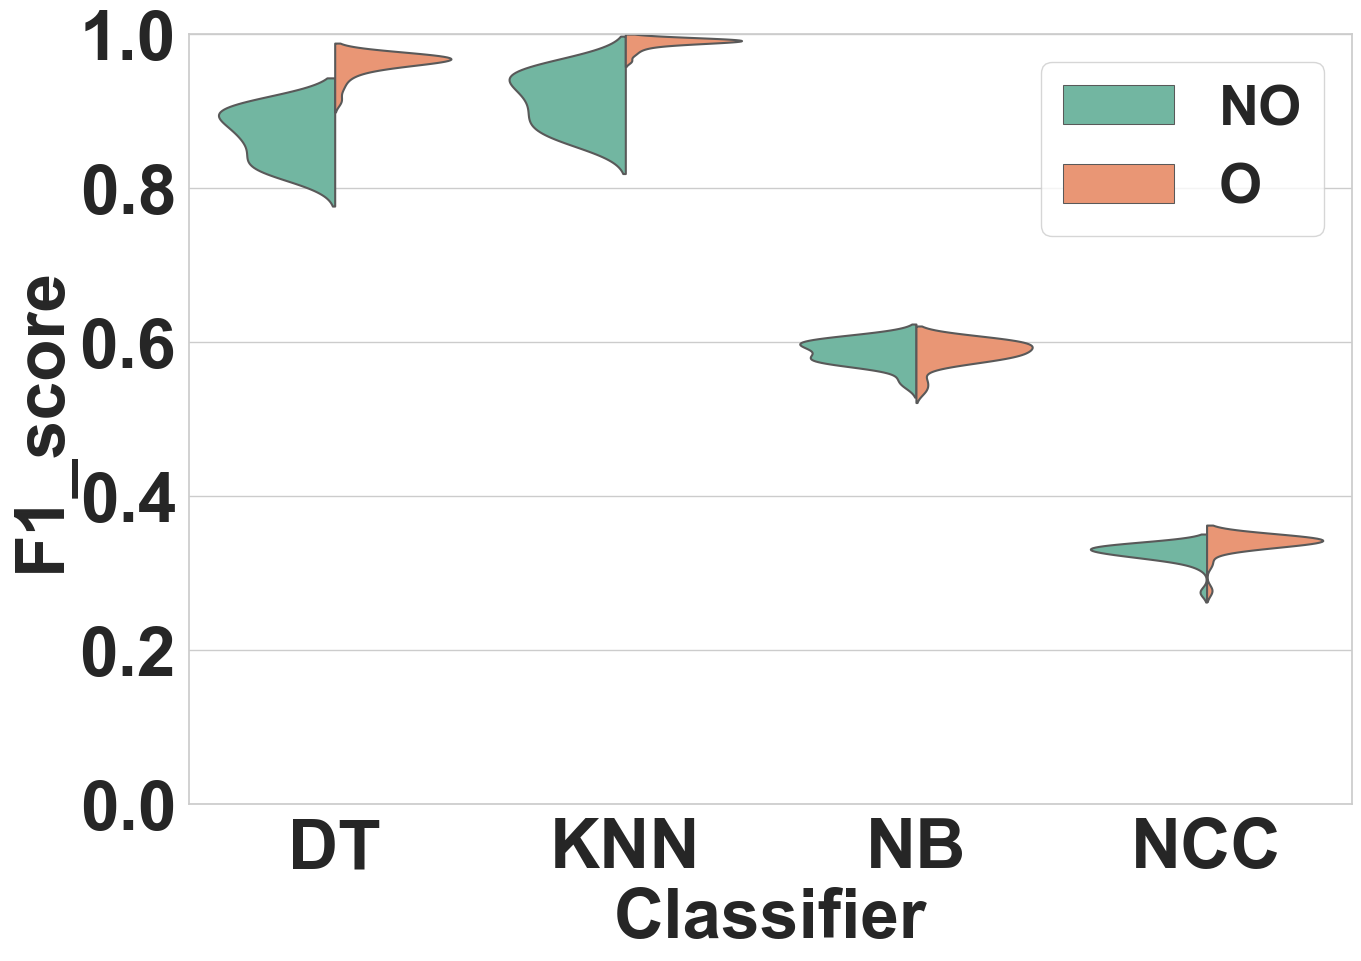
\includegraphics[scale=0.14]{Figures/Dataset1_iid_FS1.png}}\quad
  \subfigure[FS2]{\label{fig:ds1-FS2-exp1}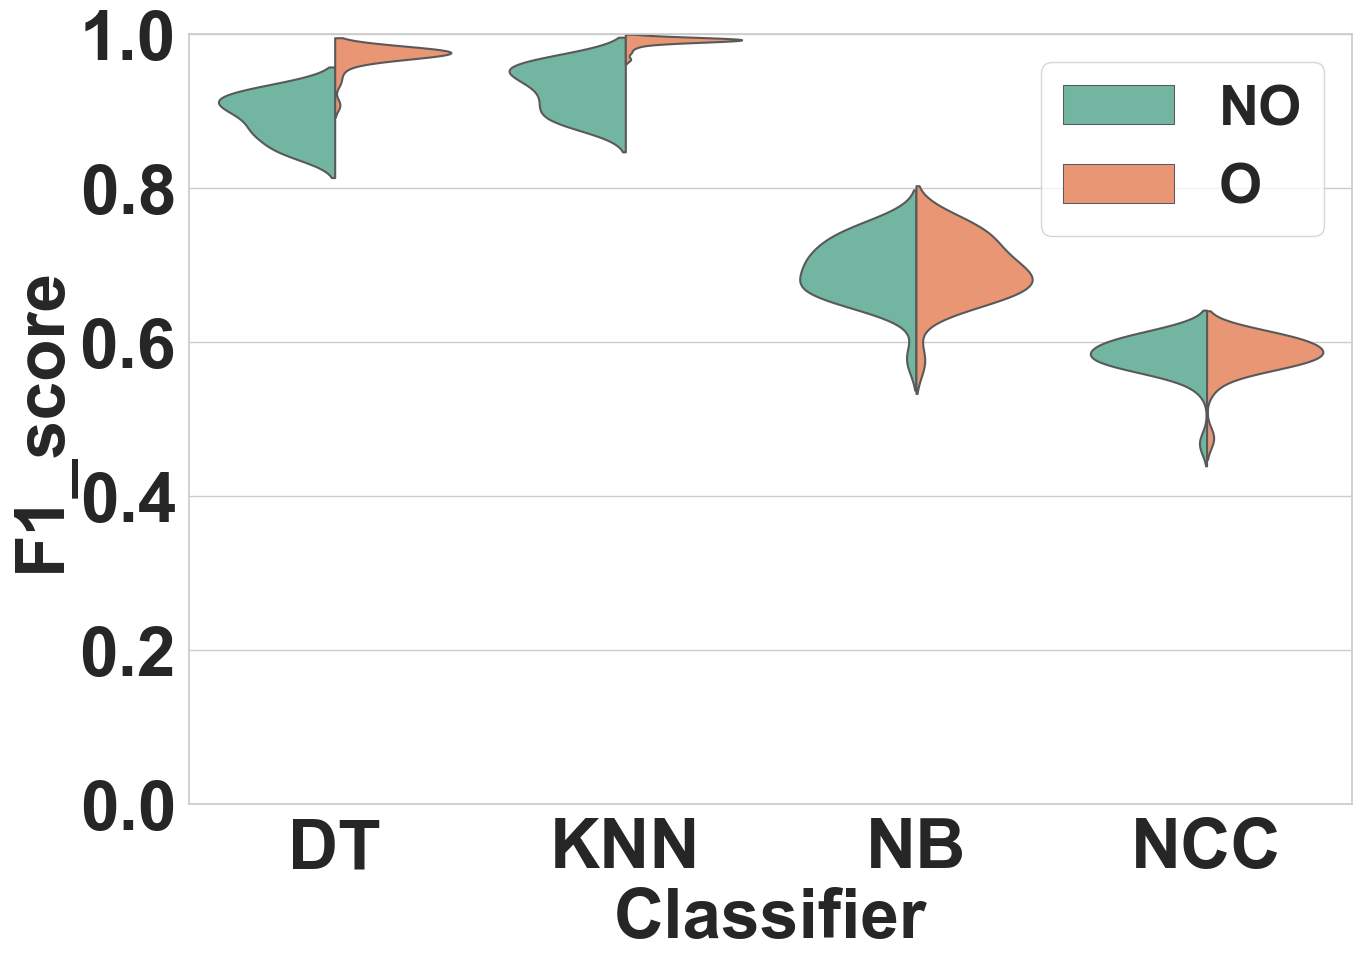
\includegraphics[scale=0.14]{Figures/Dataset1_iid_FS2.png}}
  \subfigure[FS3]{\label{fig:ds1-FS3-exp1}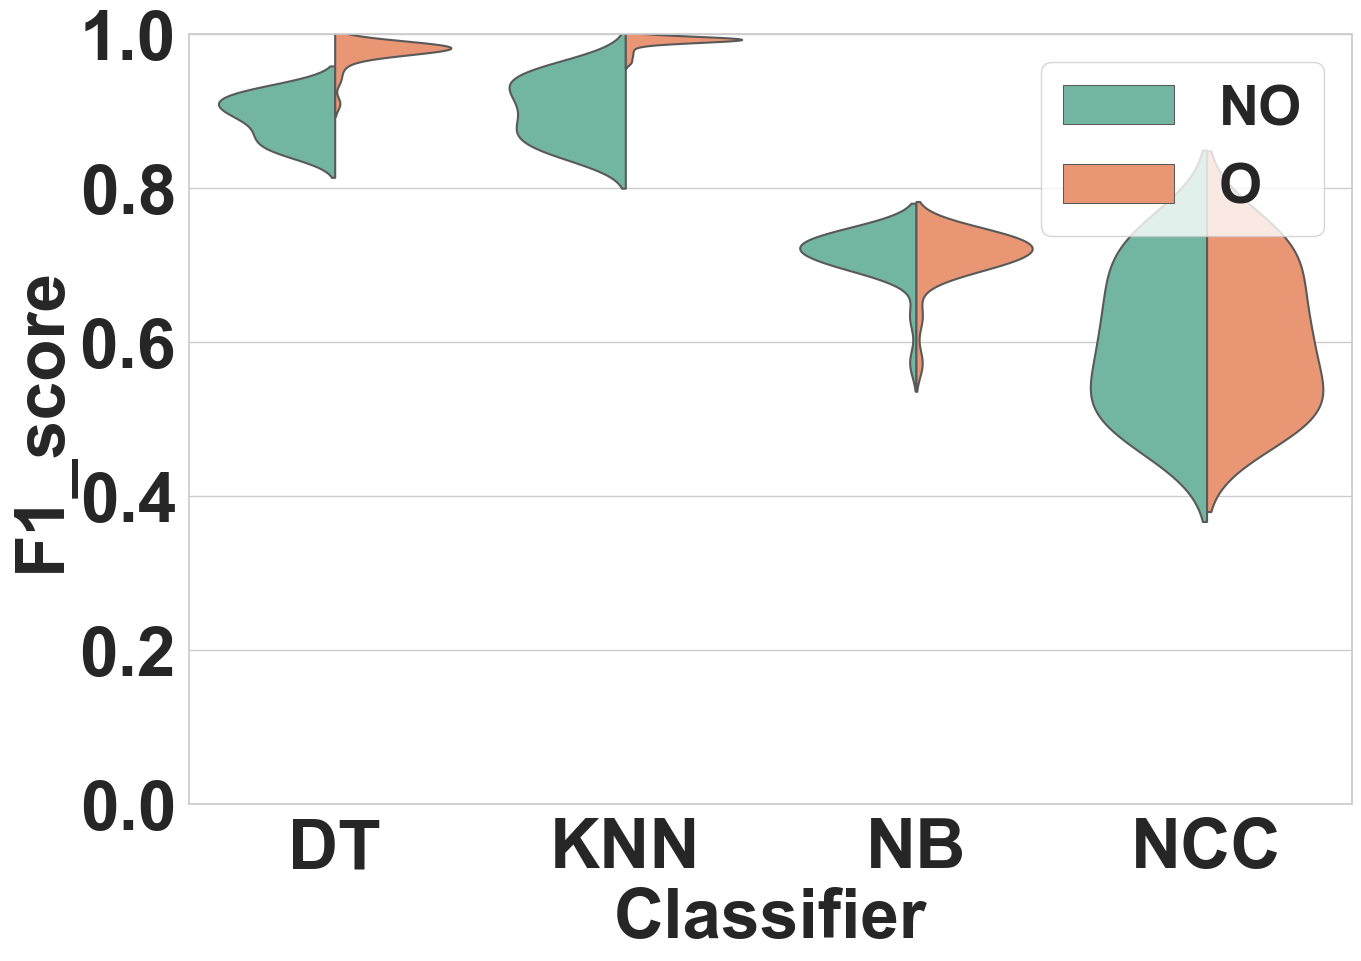
\includegraphics[scale=0.14]{Figures/Dataset1_iid_FS3.png}}
   
   \caption{Experiment 1 -- Subject-dependent CV -- Dataset 1.}
    \label{fig:exp1_ds1}
    
\end{figure}

\begin{figure}[htp]
  \centering
  \subfigure[FS1]{\label{fig:ds2-FS1-exp1}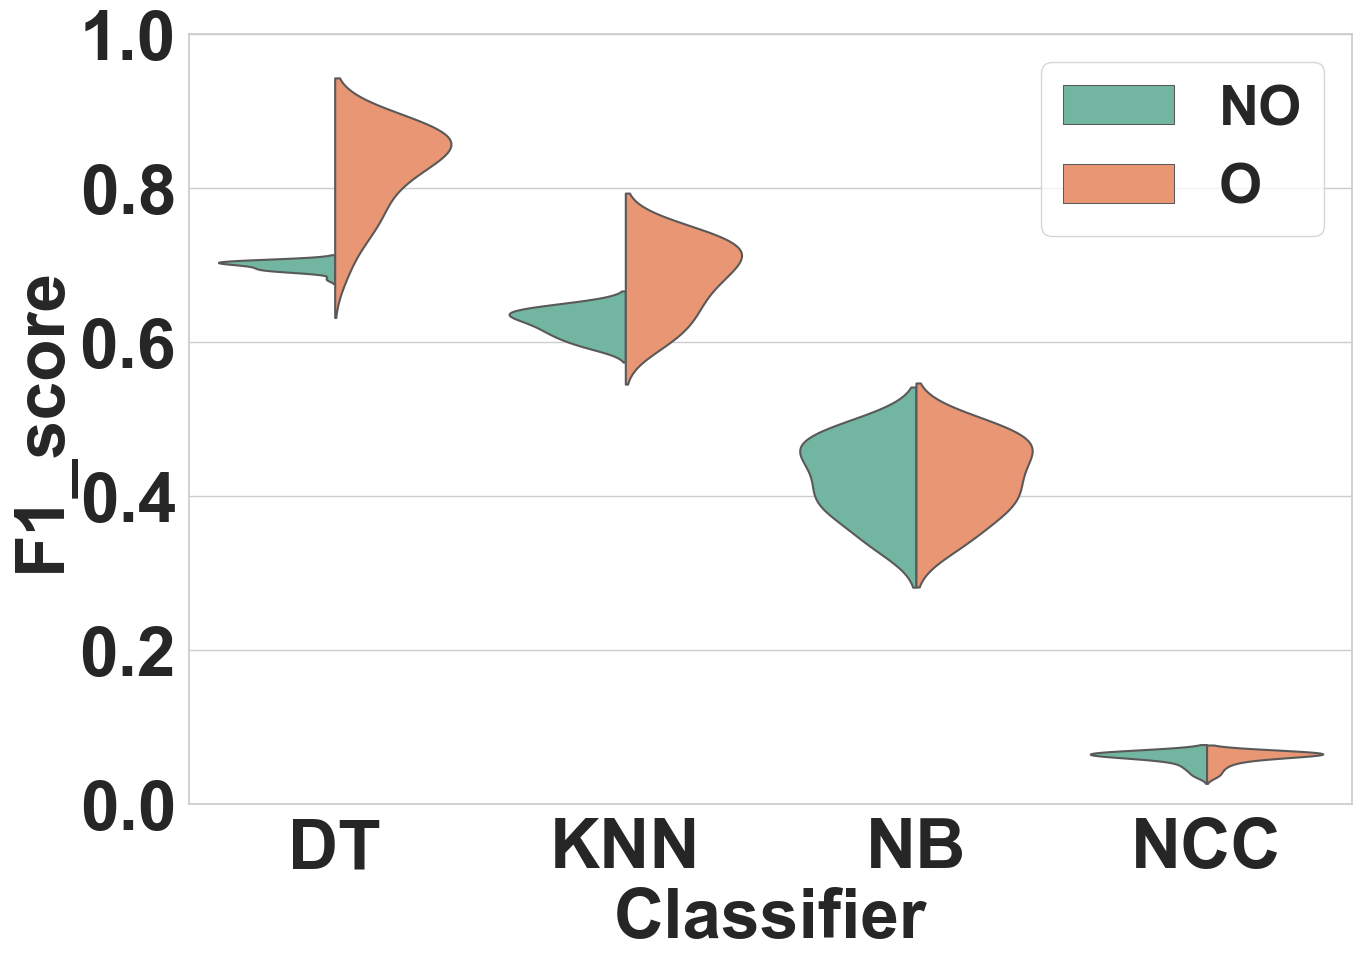
\includegraphics[scale=0.14]{Figures/Dataset2_iid_FS1.png}}\quad
  \subfigure[FS2]{\label{fig:ds2-FS2-exp1}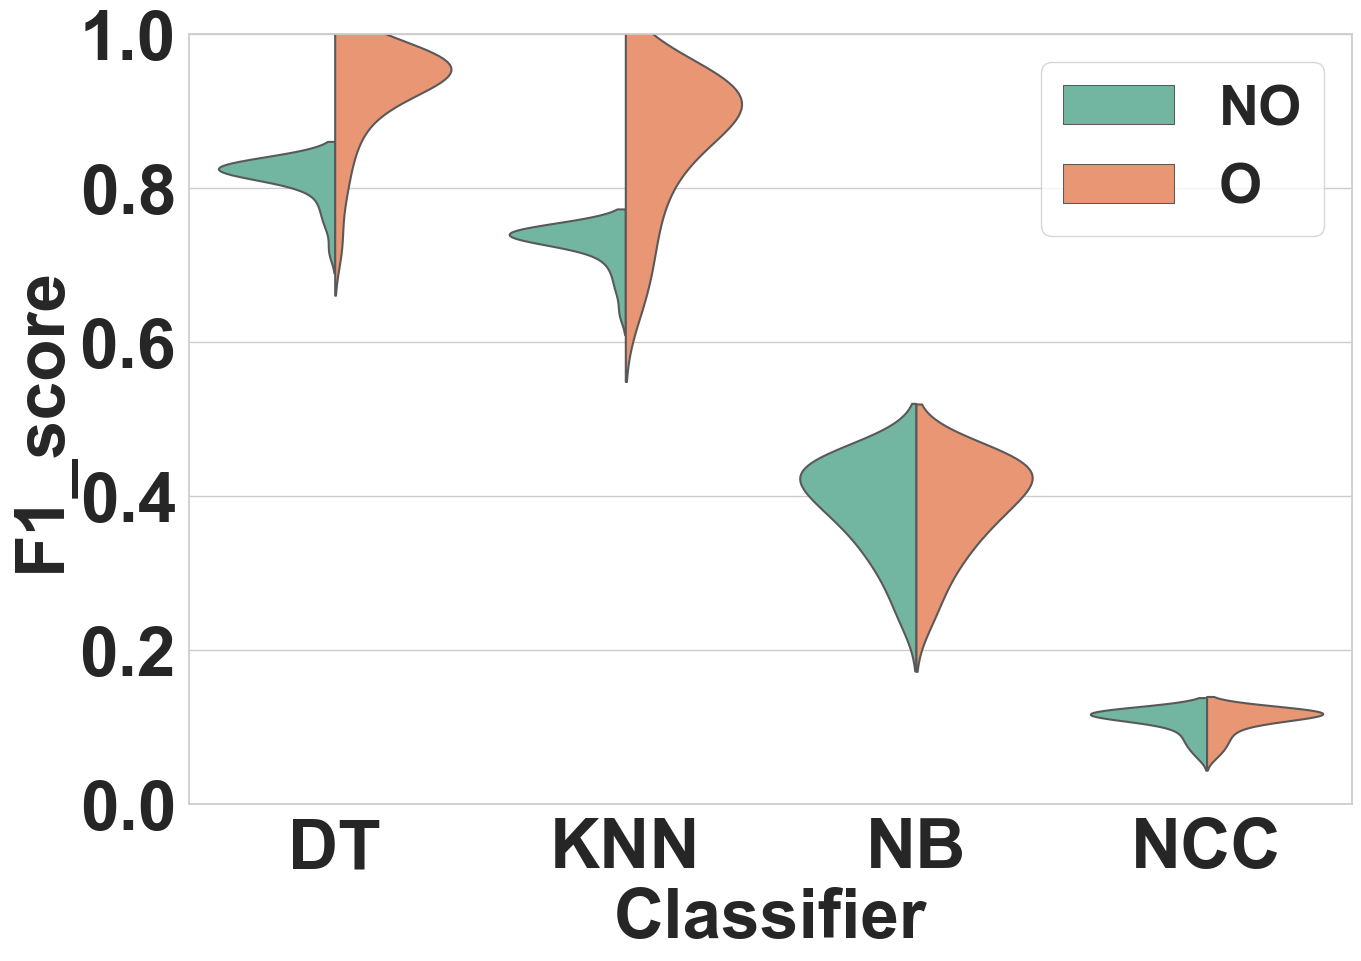
\includegraphics[scale=0.14]{Figures/Dataset2_iid_FS2.png}}
  \subfigure[FS3]{\label{fig:ds2-FS3-exp1}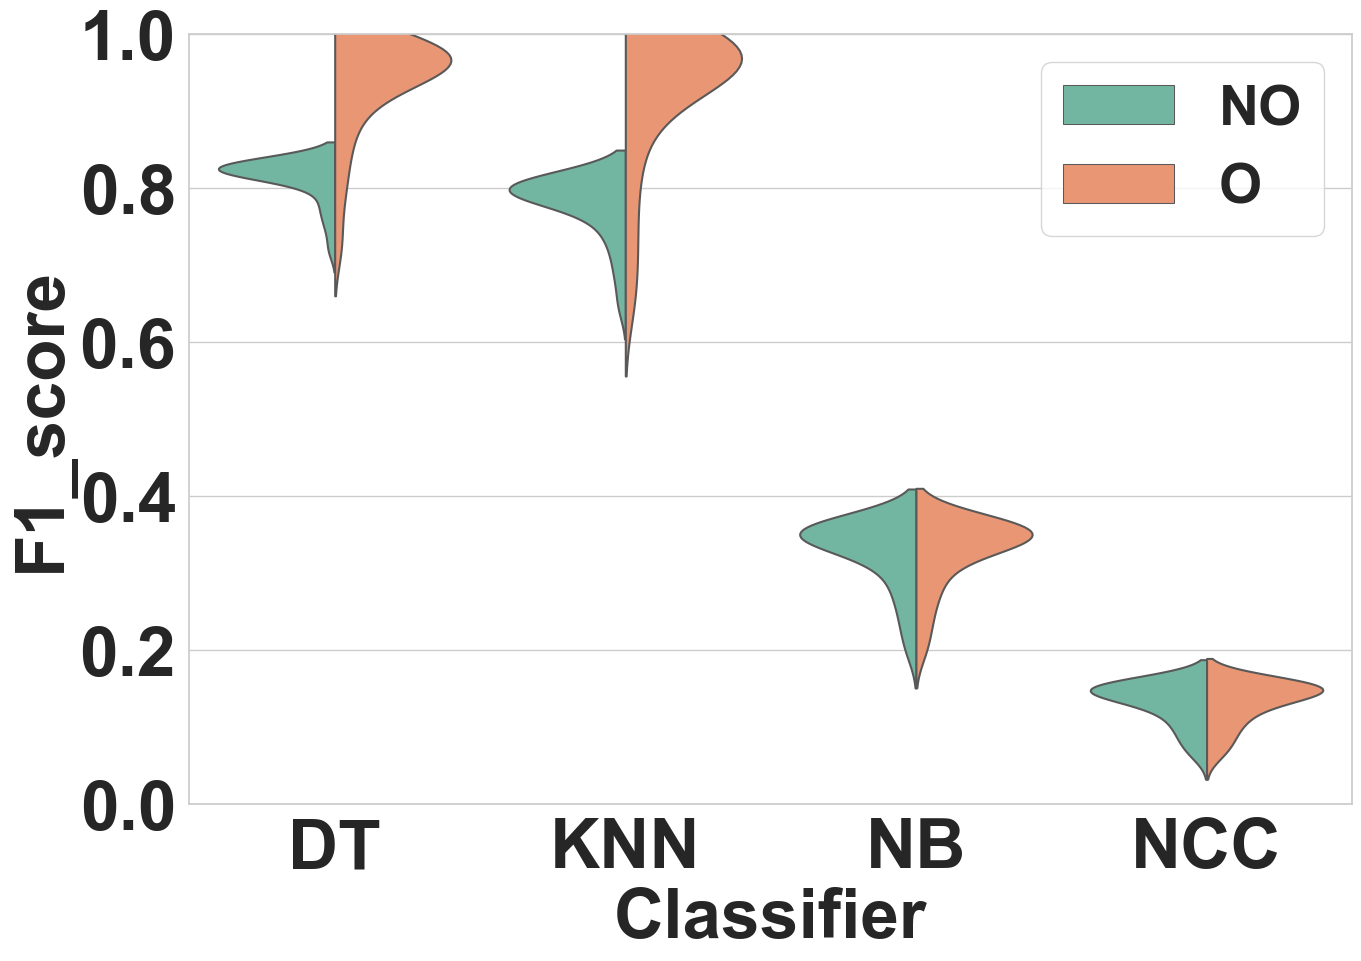
\includegraphics[scale=0.14]{Figures/Dataset2_iid_FS3.png}}
   
   \caption{Experiment 1 -- Subject-dependent CV -- Dataset 2. }
    \label{fig:exp1_ds2}
    
\end{figure}

\begin{figure}[htp]
  \centering
  \subfigure[FS1]{\label{fig:ds1-FS1-exp2}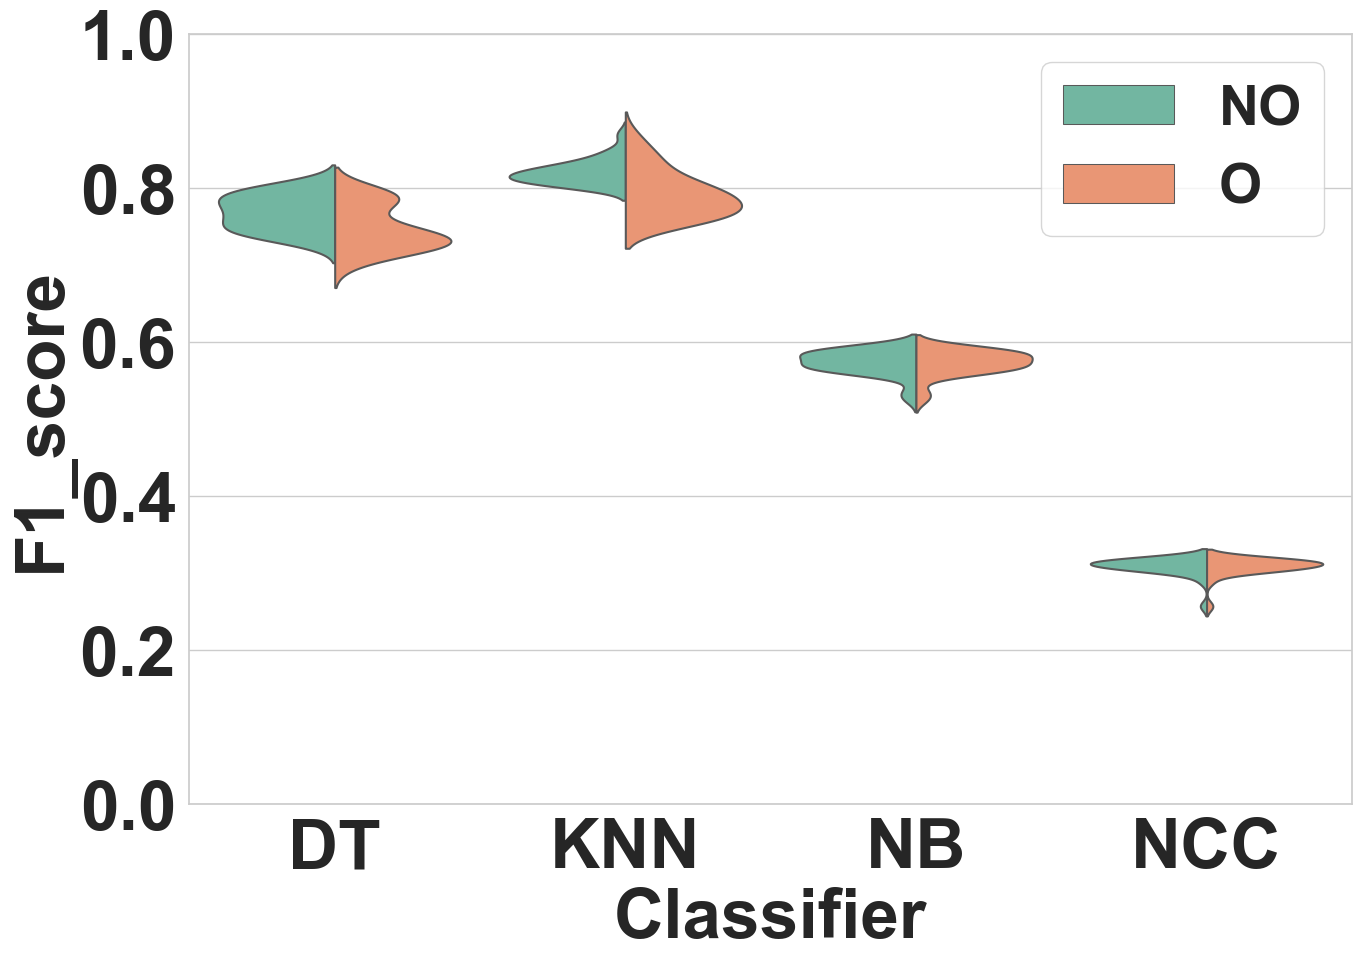
\includegraphics[scale=0.14]{Figures/Dataset1_sbj_FS1.png}}\quad
  \subfigure[FS2]{\label{fig:ds1-FS2-exp2}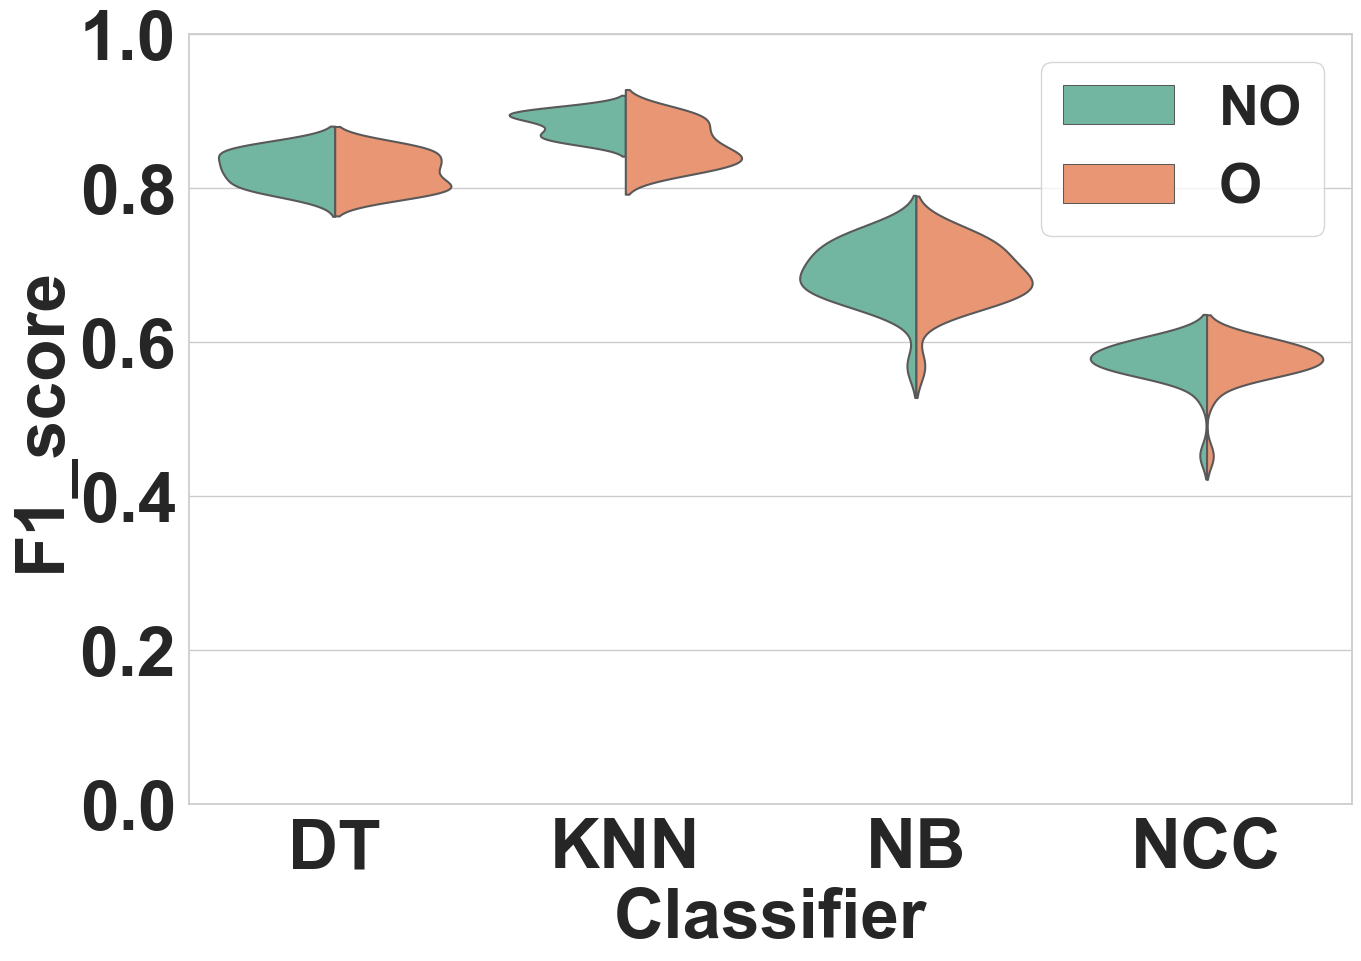
\includegraphics[scale=0.14]{Figures/Dataset1_sbj_FS2.png}}
  \subfigure[FS3]{\label{fig:ds1-FS3-exp2}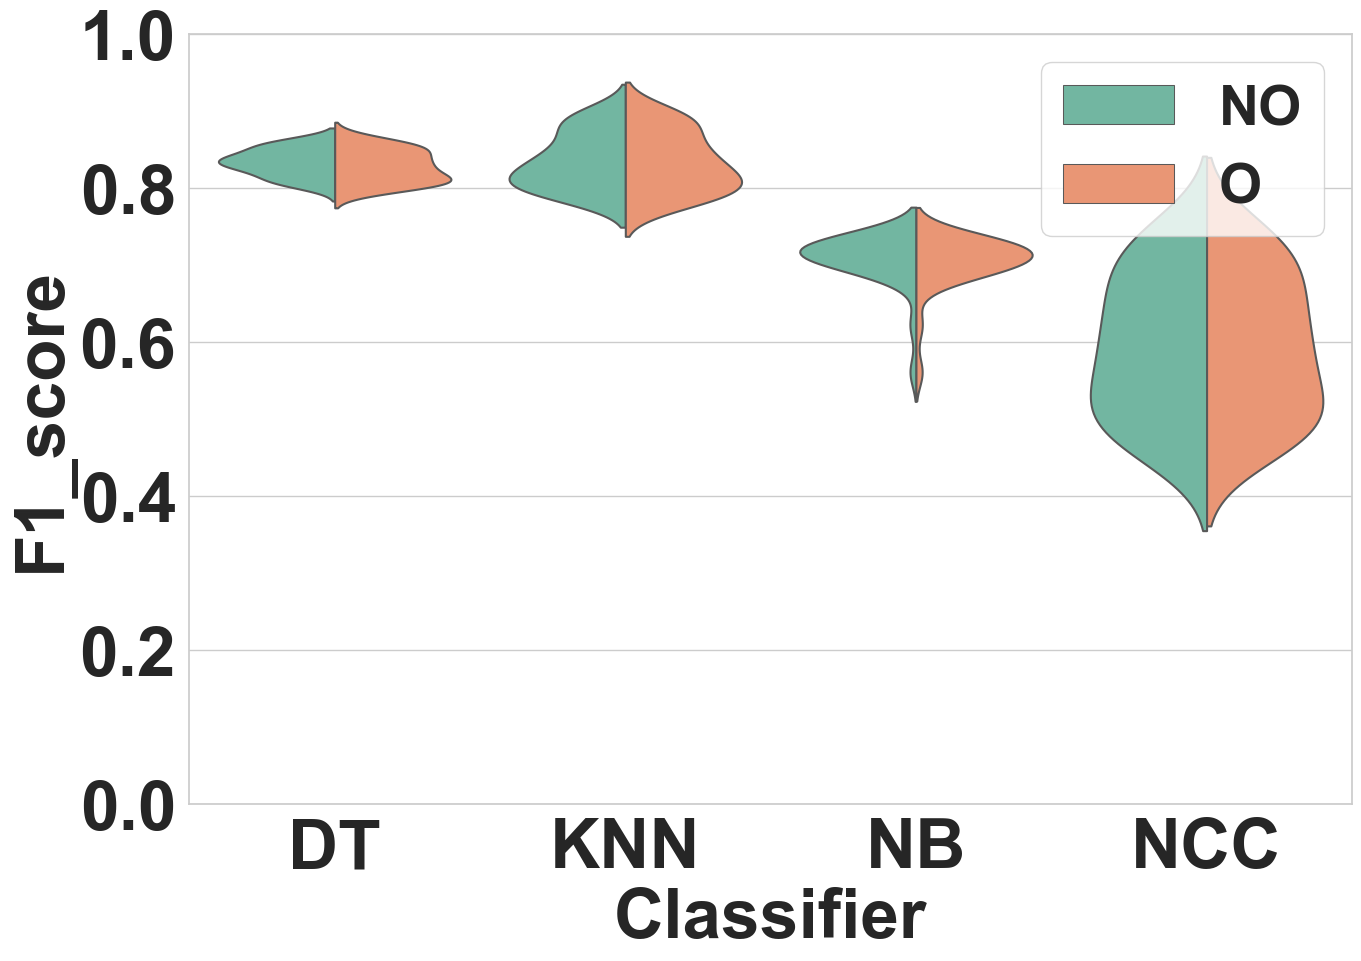
\includegraphics[scale=0.14]{Figures/Dataset1_sbj_FS3.png}}
   
   \caption{Experiment 2 -- Subject-independent CV -- Dataset 1.}
    \label{fig:exp2_ds1}
    
\end{figure}

\begin{figure}[htp]
  \centering
  \subfigure[FS1]{\label{fig:ds2-FS1-exp2}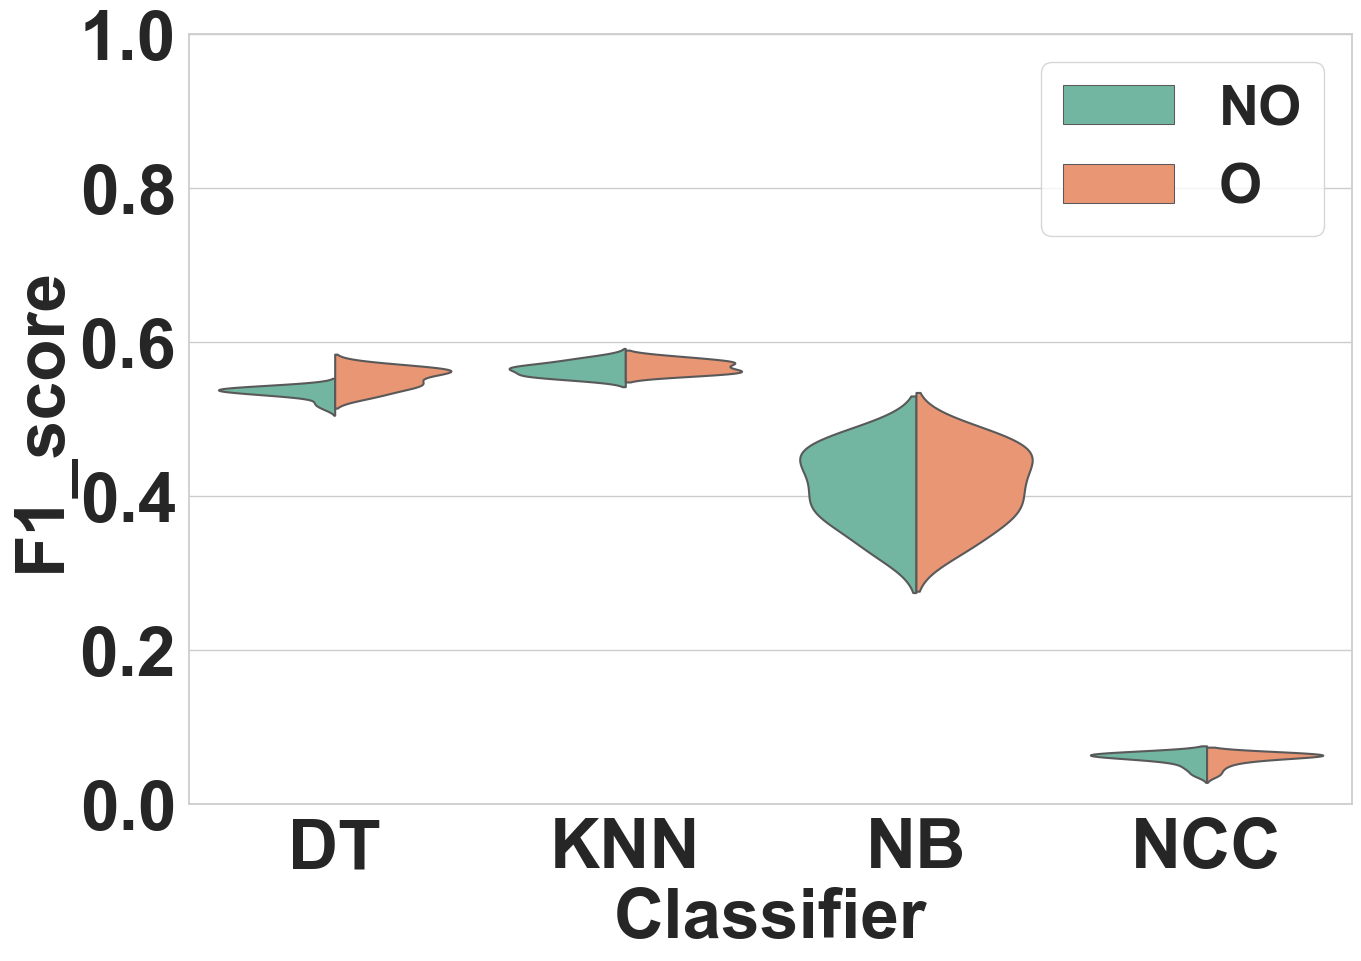
\includegraphics[scale=0.14]{Figures/Dataset2_sbj_FS1.png}}\quad
  \subfigure[FS2]{\label{fig:ds2-FS2-exp2}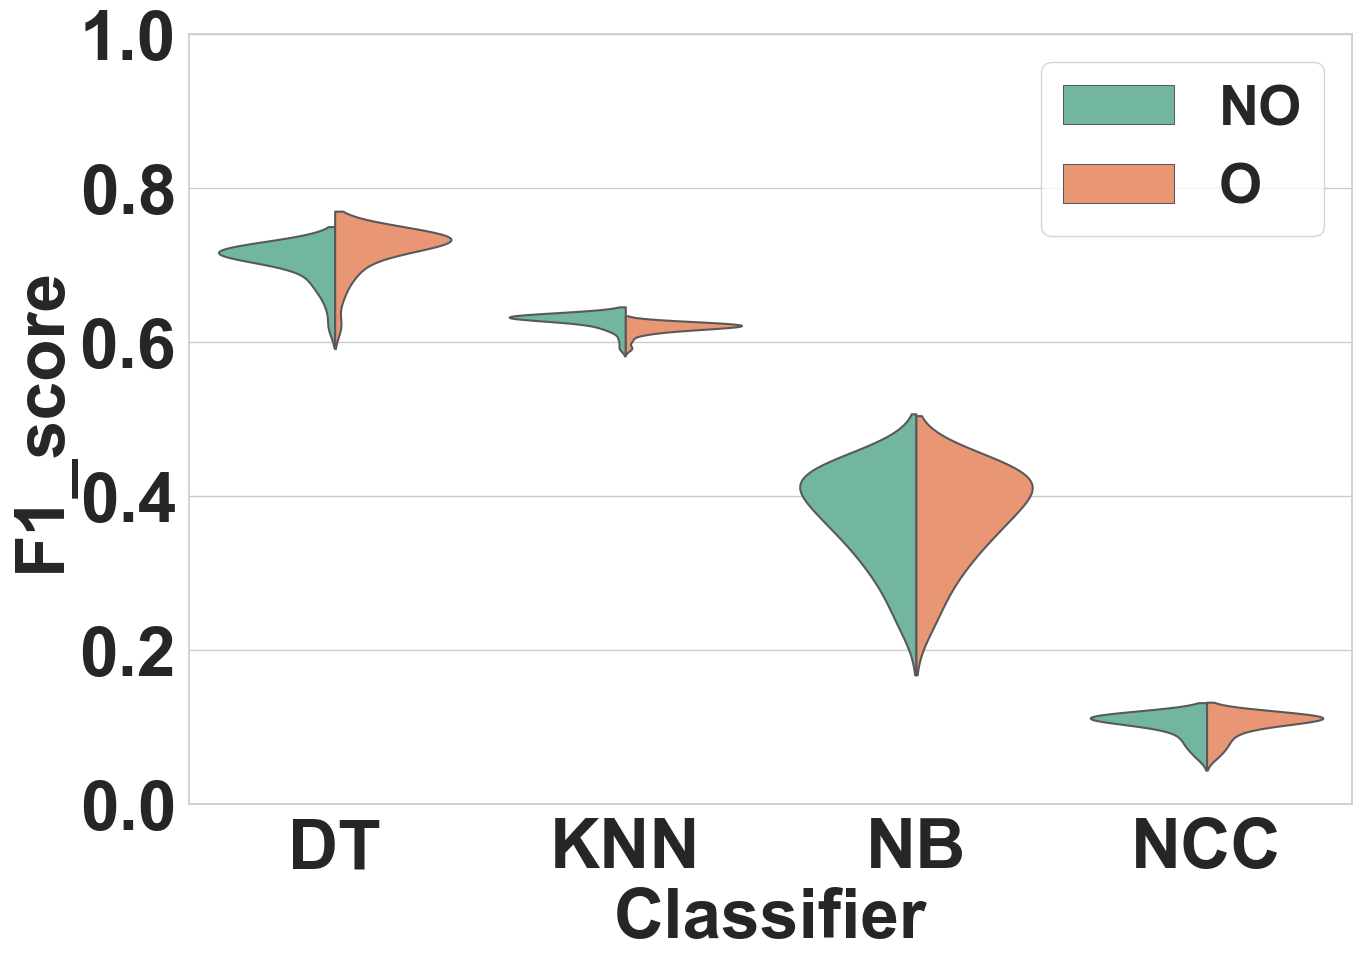
\includegraphics[scale=0.14]{Figures/Dataset2_sbj_FS2.png}}
  \subfigure[FS3]{\label{fig:ds2-FS3-exp2}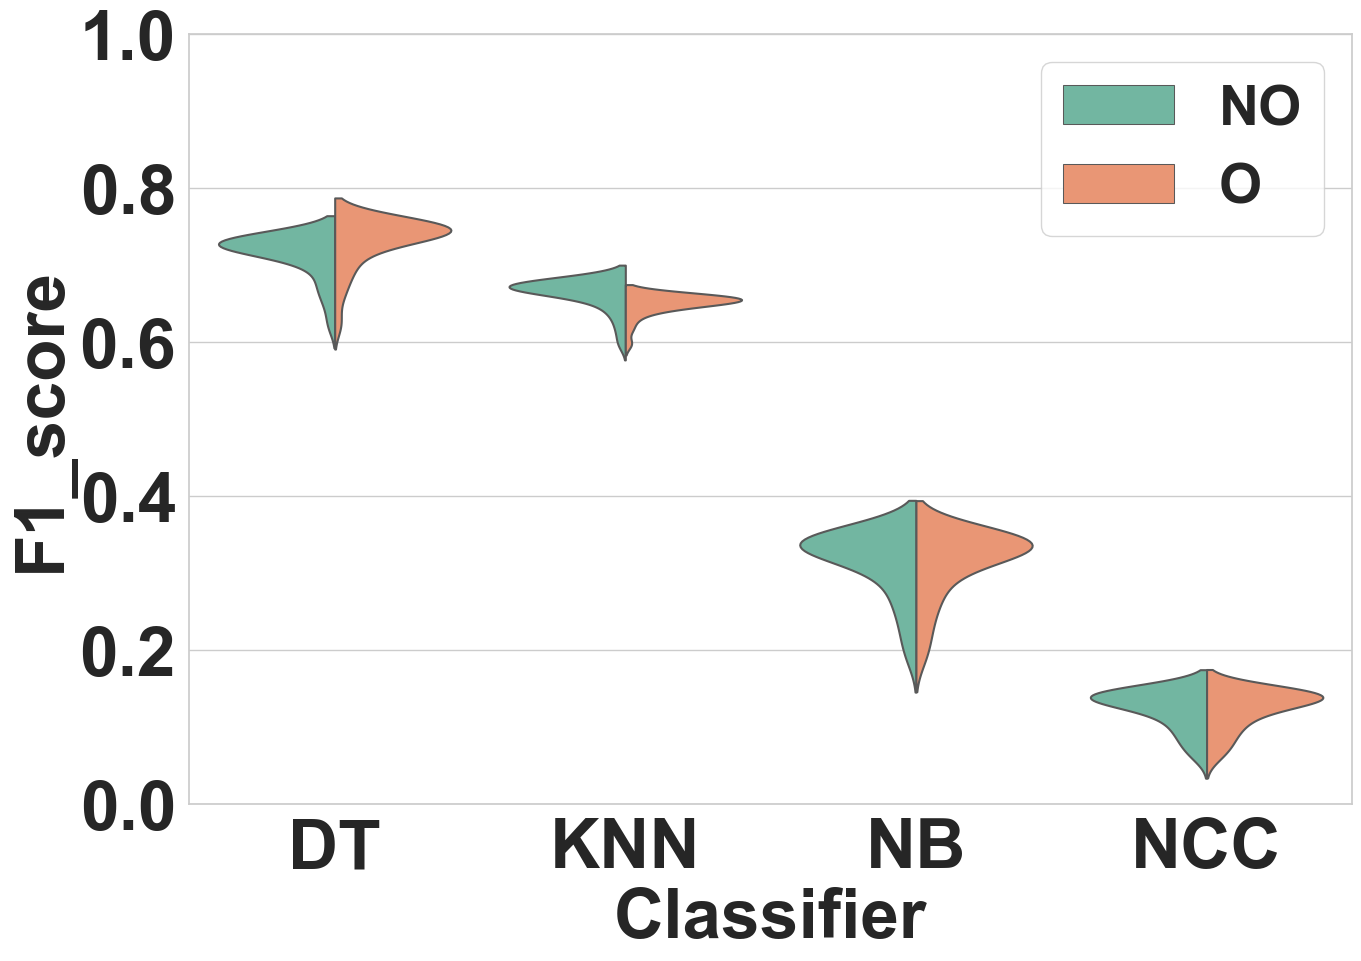
\includegraphics[scale=0.14]{Figures/Dataset2_sbj_FS3.png}}
   
   \caption{Experiment 2 -- Subject-independent CV -- Dataset 2.}
    \label{fig:exp2_ds2}
    
\end{figure}

\subsubsection{Experiment 3: Subject-independent CV and new hyperparameters } \label{sec:ex3}
One may claim that the results of Experiment~2 
are due to the specific set of hyperparameters used in the classifiers. Thus, to investigate that, we reproduced Experiment~2 with a new set of hyperparameters for the KNN and DT classifiers.

We selected new hyperparameter values such that (1) overfitting or underfitting does not occur, and (2) the new values are as different as possible from those in the previous experiments. Table~\ref{tab:hparams} compares the selected values for hyperparameters of DT and KNN in Experiment~1 and Experiment~2. 

\begin{table}[]
    \centering
\begin{tabular}{|>{}c|>{}c|>{}c|>{}c|}
\hline 
\multirow{1}{*}{Classifier} & Hyperparameter & Experiment~2 & Experiment~3\tabularnewline
\hline 
KNN & K (n\_neighbors) & 3 & 6\tabularnewline
\hline 
\multirow{3}{*}{DT} & Criterion & 'gini' & 'entropy'\tabularnewline
\cline{2-4} \cline{3-4} \cline{4-4} 
 & max\_depth & None & 20\tabularnewline
\cline{2-4} \cline{3-4} \cline{4-4} 
 & max\_features & 1 & 0.7\tabularnewline
\hline 
\end{tabular}
    \caption{The hyperparameters values for KNN and DT in Experiment~1 and Experiment~2. When max\_depth is set to None, the decision tree is expanded until all leaves are pure~\cite{pedregosa2011scikit}.}
    \label{tab:hparams}
\end{table}

\noindent\textbf{Dataset~1.} Results are shown in Figure~\ref{fig:exp3_ds1}. As in the previous experiments, the F1-scores obtained with overlapping and with non-overlapping windows are comparable. For DT, using overlapping windows decreases the performance in all feature sets, by about 1\%. As for KNN, using overlapping windowing reduces the F1-score by about 4\% in FS1 and FS2, and increases it by 1\% in FS3.   

\noindent\textbf{Dataset~2.} Figure~\ref{fig:exp3_ds2} shows our results for this dataset. The trend is similar to the previous experirments, i.e., F1-scores obtained with overlapping and with non-overlapping windowing are very similar. Qualitatively, such differences for both classifiers remain lower than 1\% in all feature sets.  

In conclusion, overlapping windowing does not provide any performance improvement compared to non-overlapping windowing with our new set of hyperparameters, which confirms the findings of Experiment 2.

% exp3 figures
\begin{figure}[htp]
  \centering
  \subfigure[FS1]{\label{fig:ds1-FS1-exp3}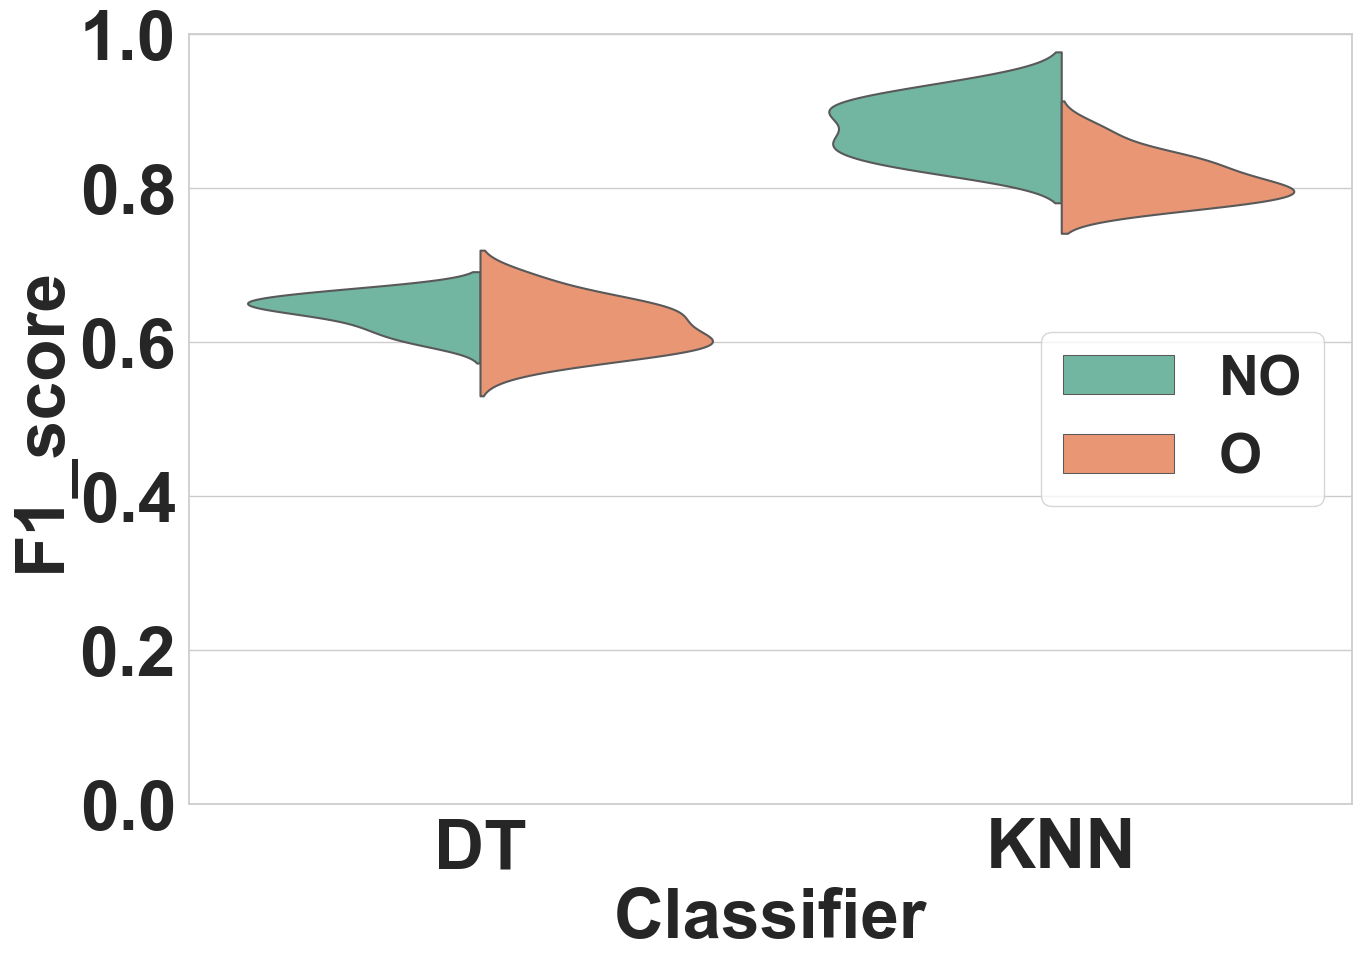
\includegraphics[scale=0.14]{Figures/Dataset1_sbj_FS1_new_hparams.png}}\quad
  \subfigure[FS2]{\label{fig:ds1-FS2-exp3}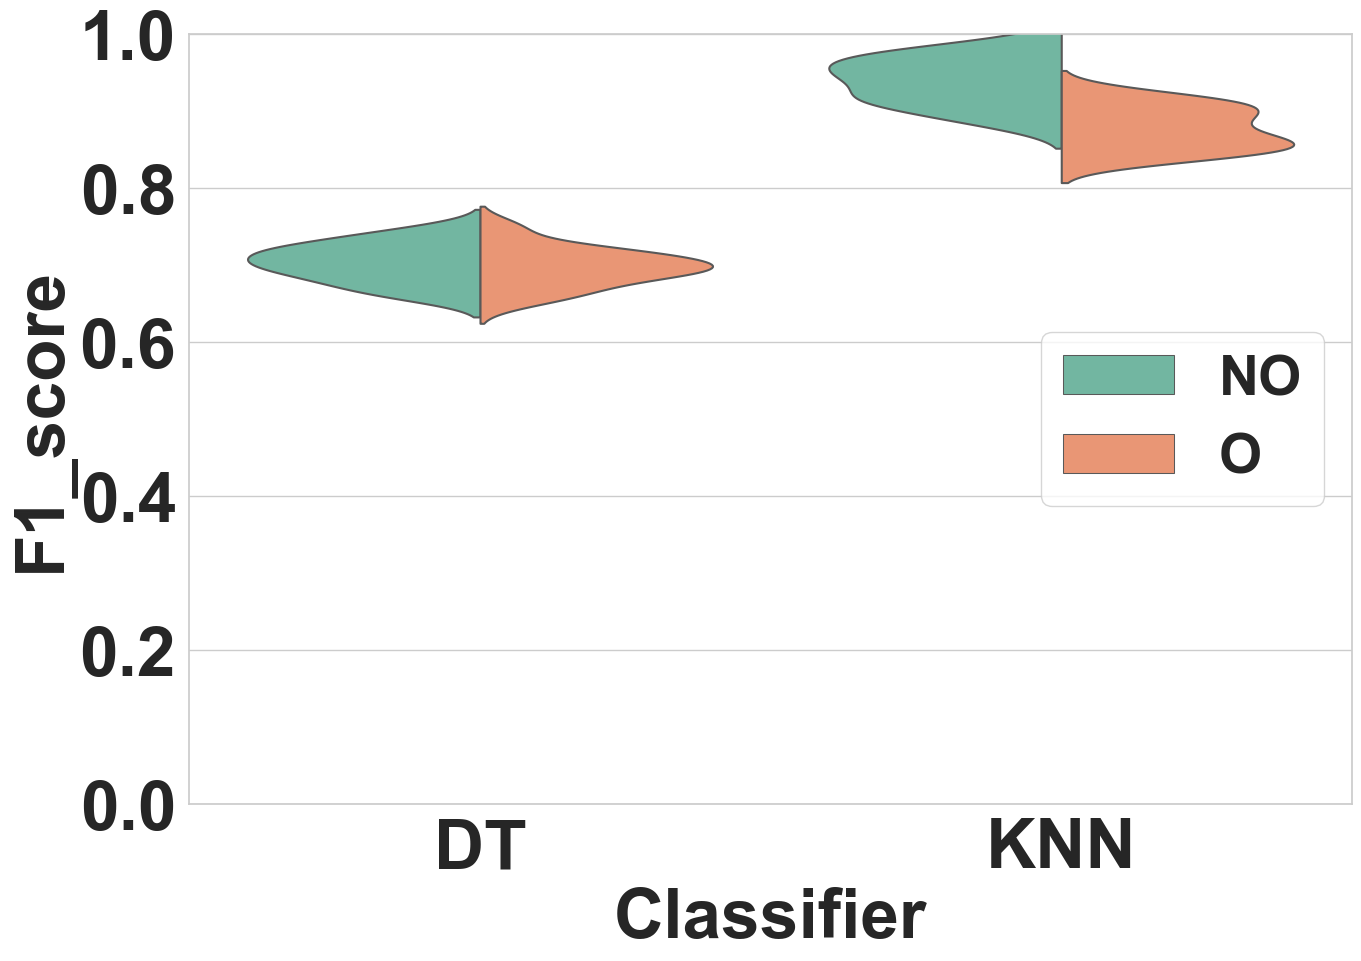
\includegraphics[scale=0.14]{Figures/Dataset1_sbj_FS2_new_hparams.png}}
  \subfigure[FS3]{\label{fig:ds1-FS3-exp3}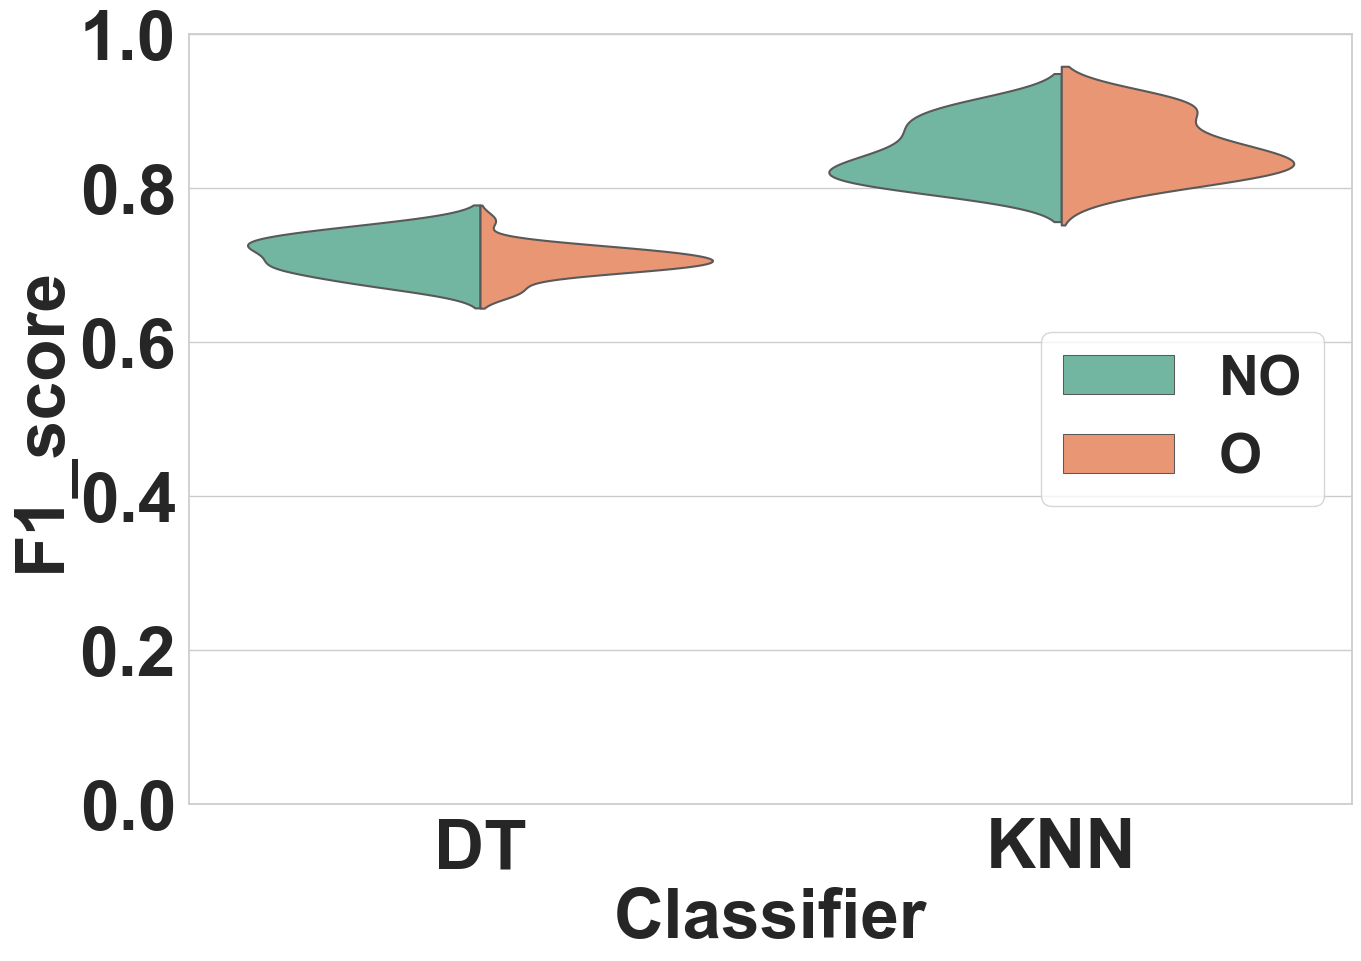
\includegraphics[scale=0.14]{Figures/Dataset1_sbj_FS3_new_hparams.png}}
   
   \caption{Experiment 3 -- Subject-independent CV -- Dataset 1.}
    \label{fig:exp3_ds1}
    
\end{figure}

\begin{figure}[htp]
  \centering
  \subfigure[FS1]{\label{fig:ds2-FS1-exp3}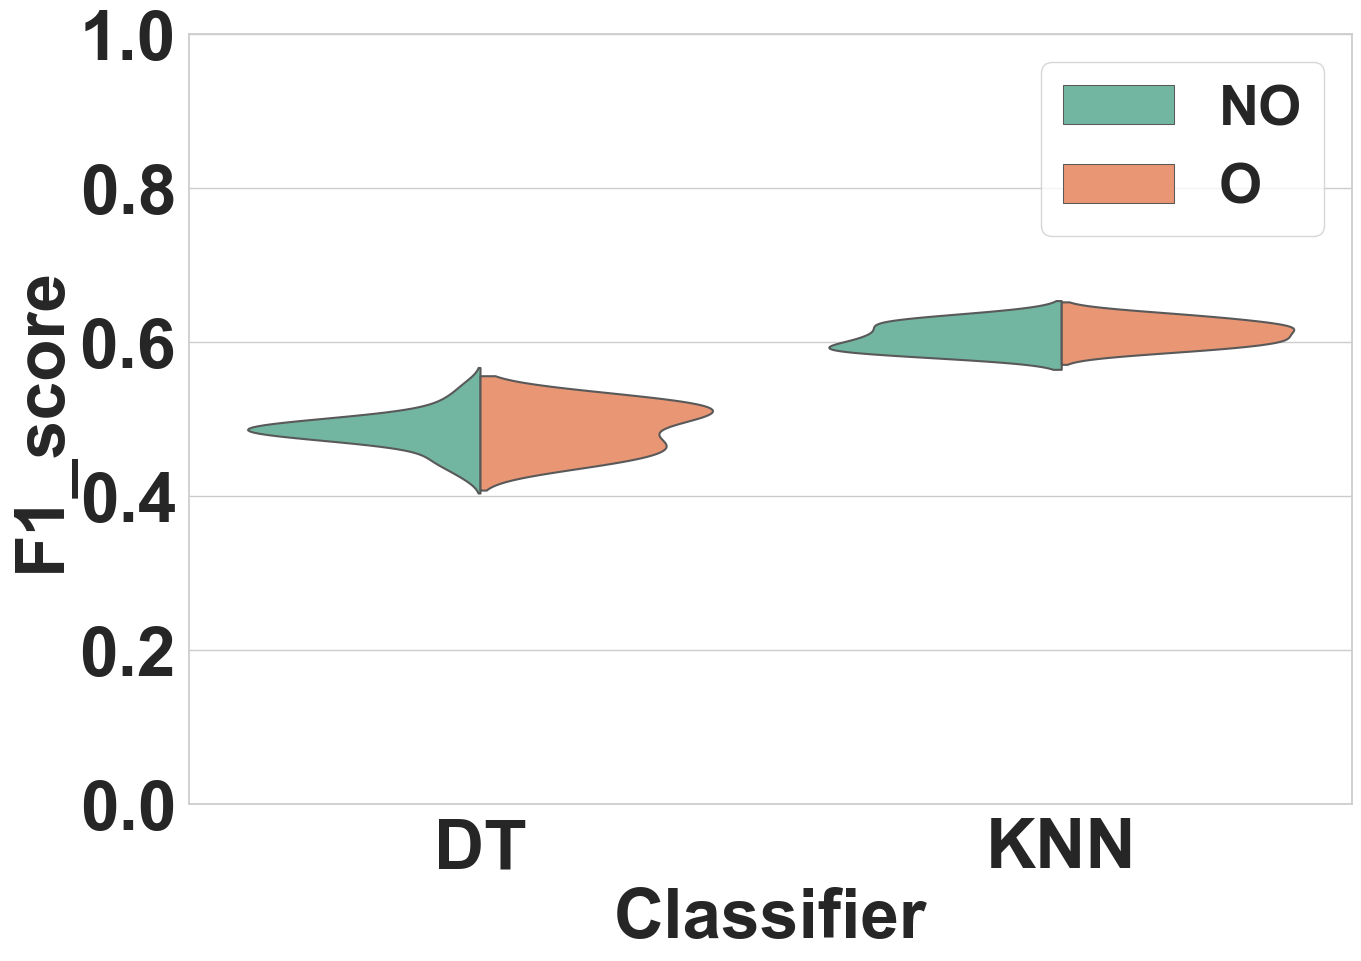
\includegraphics[scale=0.14]{Figures/Dataset2_sbj_FS1_new_hparams.png}}\quad
  \subfigure[FS2]{\label{fig:ds2-FS2-exp3}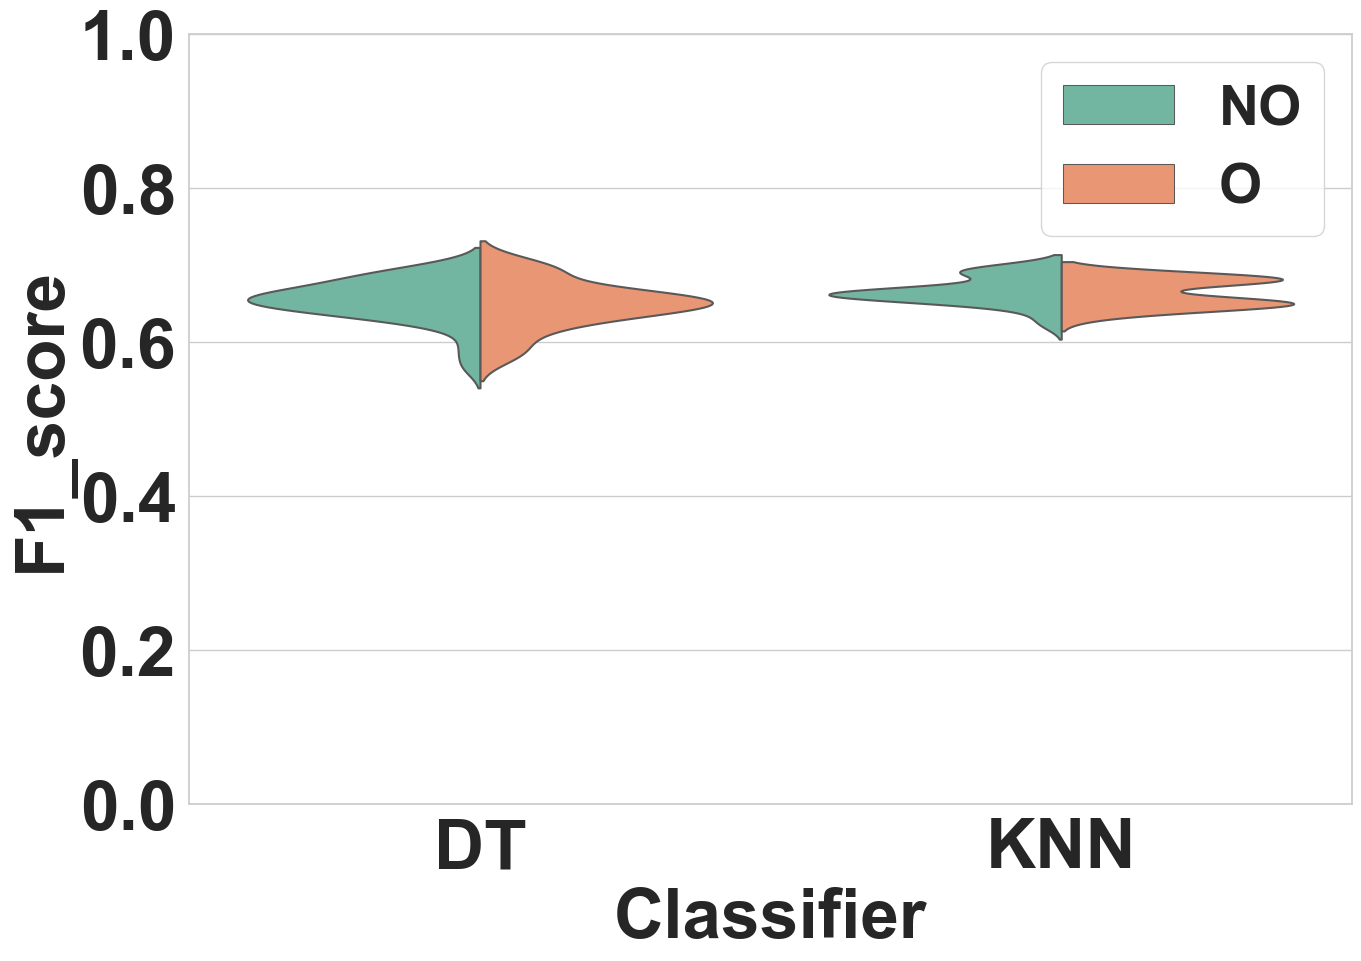
\includegraphics[scale=0.14]{Figures/Dataset2_sbj_FS2_new_hparams.png}}
  \subfigure[FS3]{\label{fig:ds2-FS3-exp3}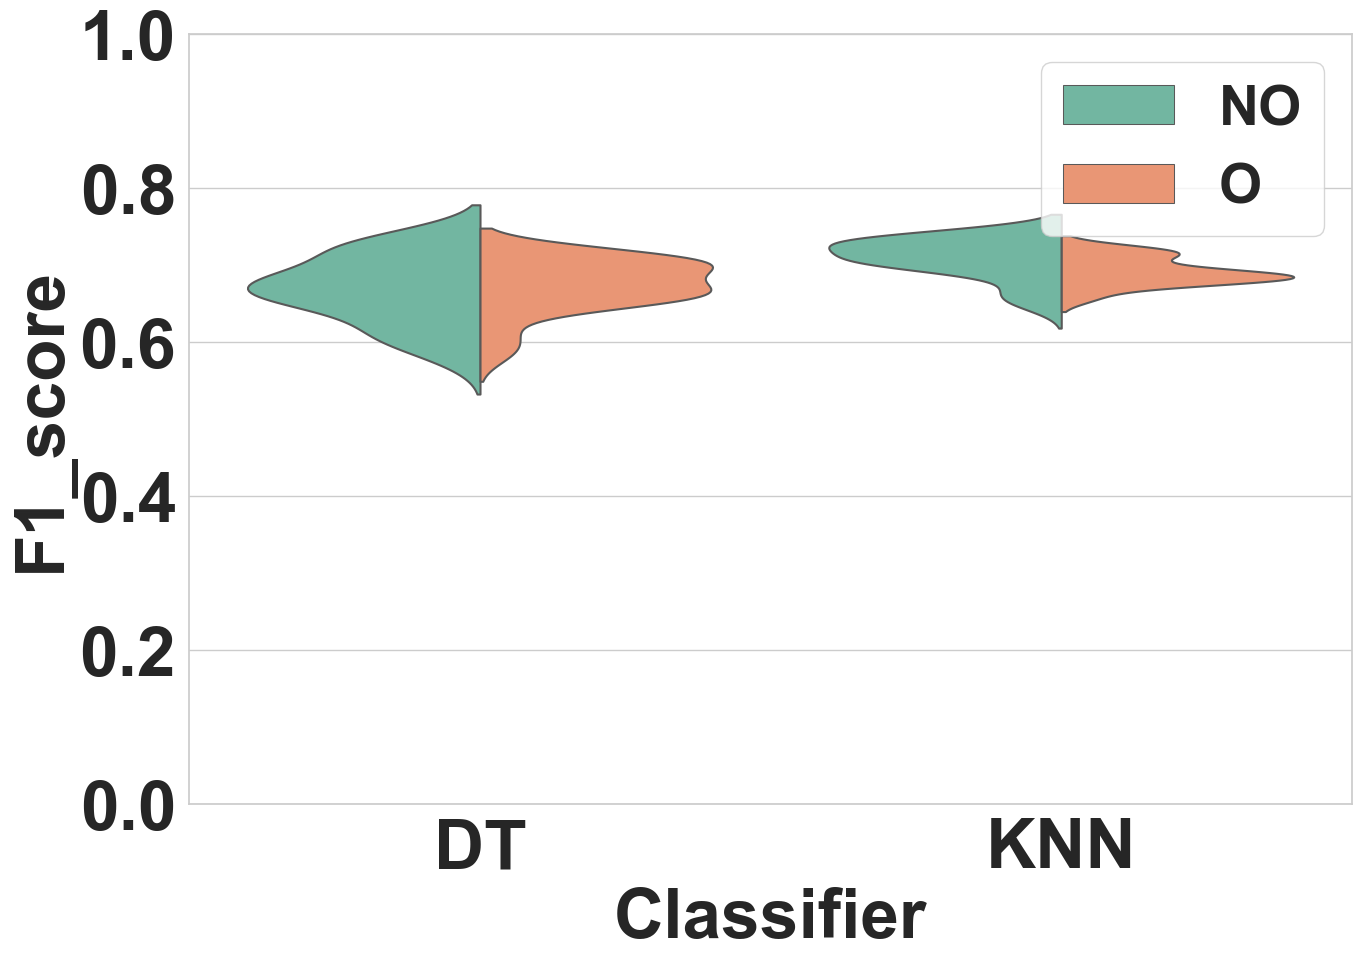
\includegraphics[scale=0.14]{Figures/Dataset2_sbj_FS3_new_hparams.png}}
   
   \caption{Experiment 3 -- Subject-independent CV -- Dataset 2.}
    \label{fig:exp3_ds2}
    
\end{figure}

\section{Activity-Specific evaluation}\label{per_activity_evaluation}
The global evaluation presented previously is useful to have a general view of the effect of windowing techniques in HAR systems. However, it is also interesting to particularize this study to each specific activity. Thus, in this section, we analyze the impact of overlapping and non-overlapping windowing for each activity.

\subsubsection{Experiment 4: Subject-independent CV per activity}
As shown by Experiment 2, overlapping and non-overlapping windowing techniques only lead to minor performance differences when evaluated with subject-independent CV. In this experiment, we investigate how this result particularize to specific activities. The presented data is the same as in Experiment 2, but the classification performance is now detailed for each activity.
For brevity, we only focus on feature set FS3. In all figures, activities are shown with the labels reported in Tables~\ref{tab:Activites1} (Dataset 1) and Tables~\ref{tab:Activites2} (Dataset 2).  

\noindent\textbf{Dataset~1.} In Figure~\ref{fig:exp5_ds1}, the activity-specific F1-scores distributions achieved for all classifiers, window sizes and windowing approaches are presented. As expected from the results shown in~\ref{fig:ds1-FS3-exp2}, the differences between overlapping and non-overlapping windowing for all activities are slow. In general, the performances of the majority of the activities drop (by 5\% on average) when overlapping windowing is used instead of non-overlapping windowing. However, using DT (Figure~\ref{fig:DT_ds1-activity-exp5}), some activities such as Heels  (27), Rotation on knees (30), Trunk Twist (10), Knees (altering) (26), Knees Bending (28), Rowing (31) and Jump rope (8) show a small performance improvement by overlapping windowing.  As for KNN (Figure~\ref{fig:KNN_ds1-activity-exp5}), performance reductions resulting from the use of overlapping windowing are higher than for DT. As an example, using overlapping drops the performance of activity Repetitive forward stretching (17) by 11\%. This may be due to the nature of KNN~\cite{cover1967nearest}, for which a small change in the dataset may have a large impact on the performance. Similar to DT, the performance for some activities also improves when overlapping windows are used, but by less than 2\%. As can be seen in Figure~\ref{fig:NB_ds1-activity-exp5} and Figure~\ref{fig:NCC_ds1-activity-exp5}, the performance of all activities for NB and NCC are almost the same.    



\noindent\textbf{Dataset~2.} Our results for this experiment are shown in Figure~\ref{fig:exp5_ds2}. 

Similar to Dataset~1, the activity-specific F1-score distributions obtained for this dataset for the two scenarios are similar. For this dataset, using overlapping windowing with KNN and DT slightly enhances the F1-score of the majority of activities in comparison to non-overlapping windowing, by 4\% on average. The highest improvements are observed for activities Lawnmower (right) (21), Lateral Raise (19) and Seated Back Fly (31) for DT and for Wall Ball (40), Seated Back Fly (31) and Power Boat pose (26) for KNN. Similar to Dataset~1, the performance of NB and NCC for all activities in both scenarios are almost the same.

This experiment shows that using overlapping windowing with subject-independent validation can impact the recognition performance of HAR systems for diverse activities differently. In spite of being mostly minor, for the activities in this study, overlapping windowing reduces the recognition accuracy of most activities and only a few of them shows improvement. Moreover, the impact of overlapping windowing may be subject to the dataset, i.e., using overlapping windowing may impact the performance of the system in recognizing a single activity in different way. Running is a good example here. Using overlapping windowing reduces the F1-score of the system for this activity in Dataset~1, but it improves that in Dataset~2.  

In summary, the recognition accuracy for most of the activities investigated in this study is quite comparable between the two scenarios with overlapping and non-overlapping windows.    

\subsubsection{Experiment 5: More discriminative features and neural-network classifier}
In this experiment, we evaluate the effectiveness of non-overlapping windows using more discriminative time-domain features and a custom fine-tuned classifier. Namely, we target the HAR framework presented in~\cite{omid2019MPR}. The approach in~\cite{omid2019MPR} utilizes configurable time-domain histogram features and a single hidden layer neural network classifier. It has been shown that the framework can outperform KNN classifiers as well as many other time-domain features explored by previous work. The framework in~\cite{omid2019MPR} allows for a segmentation with a configurable sliding window. It presents results on subject independent cross validation using Dataset~2 and a 5s overlapping window sliding at 200ms steps. Here, we conduct a similar experiment, but with a non-overlapping window size of 5s. To provide a fair comparison, we use the same experimental setup compared to ~\cite{omid2019MPR}, which is presented next. 

We use time-domain histogram features, i.e., 120 bins in total, where 20 bins are assigned uniformly to each individual sensor axis. The accelerometer full-scale range has been set to $\pm{2g}$, while the gyroscope full-scale range has been set to $\pm{512dps}$. The single-hidden-layer neural network classifier consists of 120 input neurons, 60 hidden neurons and 7 output neurons targeting 6 activities and one noise class representing all other activities and the no activity periods. The Sigmoid (Softmax) trigger function has been used for the the hidden (output) layer. Training the neural network has been done in Tensorflow 1.12.0 using a batch size of 32, and the AdamOptimizer algorithm. The number of epochs is chosen, such that the overall number of data points that are fed to the neural network for training becomes identical compared to the experiment in~\cite{omid2019MPR}, i.e., similar training time. 

The normalized confusion matrix for both overlapping and non-overlapping windows under a subject-independent CV process is shown in Table~\ref{tab:MPR Comparison}. The rows refer to the true activities, while the columns correspond to the predicted ones. Each entry in the confusion matrix has two values, where the top value refers to the scenario with overlapping windows, while the bottom value corresponds to the scenario with non-overlapping windows. The results indicate that the use of overlapping windows provides minor improvements on recognition accuracy compared to the non-overlapping windows under subject independent cross validation, even when discriminative features and a well-trained neural network classifier are utilized.

%  start of Table3
\begin{table}
  \centering
\begin{tabular}{|>{}c|>{}c|>{}c|>{}c|>{}c|>{}c|>{}c|>{}c|}
\hline 
Activities & Noise (Others) & Curl & Triceps & Run & Elliptical & JumpJacks & Kettlebell\tabularnewline
\hline 
Noise (Others) & \makecell{\textbf{0.99407} \\ \textbf{0.9928}} & \makecell{0.00094 \\ 0.00103} & \makecell{0.00091 \\ 0.00099} & \makecell{0.00209 \\ 0.00286} & \makecell{0.00127 \\ 0.00129} & \makecell{0.00026 \\ 0.00028} & \makecell{0.00045 \\ 0.00074}\tabularnewline
\hline 
Curl & \makecell{0.1426 \\ 0.1369} & \makecell{\textbf{0.85082} \\ \textbf{0.8492}} & \makecell{0.00659 \\ 0.0139} & \makecell{0 \\ 0} & \makecell{0 \\ 0} & \makecell{0 \\ 0} & \makecell{0 \\ 0}\tabularnewline
\hline
Triceps & \makecell{0.17235 \\ 0.19643} & \makecell{0.00451 \\ 0.00487} & \makecell{\textbf{0.82315} \\ \textbf{0.7987}} & \makecell{0 \\ 0} & \makecell{0 \\ 0} & \makecell{0 \\ 0} & \makecell{0 \\ 0}\tabularnewline
\hline
Run & \makecell{0.20903 \\ 0.20127} & \makecell{0 \\ 0} & \makecell{0 \\ 0} & \makecell{\textbf{0.78668} \\ \textbf{0.79237}} & \makecell{0.00429 \\ 0.00565} & \makecell{0 \\ 0} & \makecell{0 \\ 0.00071}\tabularnewline
\hline
Elliptical & \makecell{0.16742 \\ 0.16265} & \makecell{0 \\ 0} & \makecell{0 \\ 0} & \makecell{0.00916 \\ 0.03113} & \makecell{\textbf{0.82342} \\ \textbf{0.80622}} & \makecell{0 \\ 0} & \makecell{0 \\ 0}\tabularnewline
\hline
JumpJacks & \makecell{0.20147 \\ 0.23729} & \makecell{0 \\ 0} & \makecell{0 \\ 0} & \makecell{0 \\ 0} & \makecell{0 \\ 0} & \makecell{\textbf{0.79853} \\ \textbf{0.76271}} & \makecell{0 \\ 0}\tabularnewline
\hline
Kettlebell & \makecell{0.18938 \\ 0.21484} & \makecell{0.00287 \\ 0} & \makecell{0 \\ 0} & \makecell{0 \\ 0} & \makecell{0 \\ 0} & \makecell{0 \\ 0} & \makecell{\textbf{0.80775} \\ \textbf{0.78516}}\tabularnewline
\hline
\end{tabular}
    \caption{Normalized confusion matrix for Experiment 5, i.e., six activities and one noise class representing all other activities and no activity periods from Dataset 2 under subject independent cross validation. Rows are true activities, and columns are predicted ones. Each entry has two values, where the top (bottom) value refers to the scenario with overlapping (non-overlapping) windows.}
    \label{tab:MPR Comparison}
\end{table}

\begin{figure}[htp]
  \centering
  \subfigure[DT]{\label{fig:DT_ds1-activity-exp5}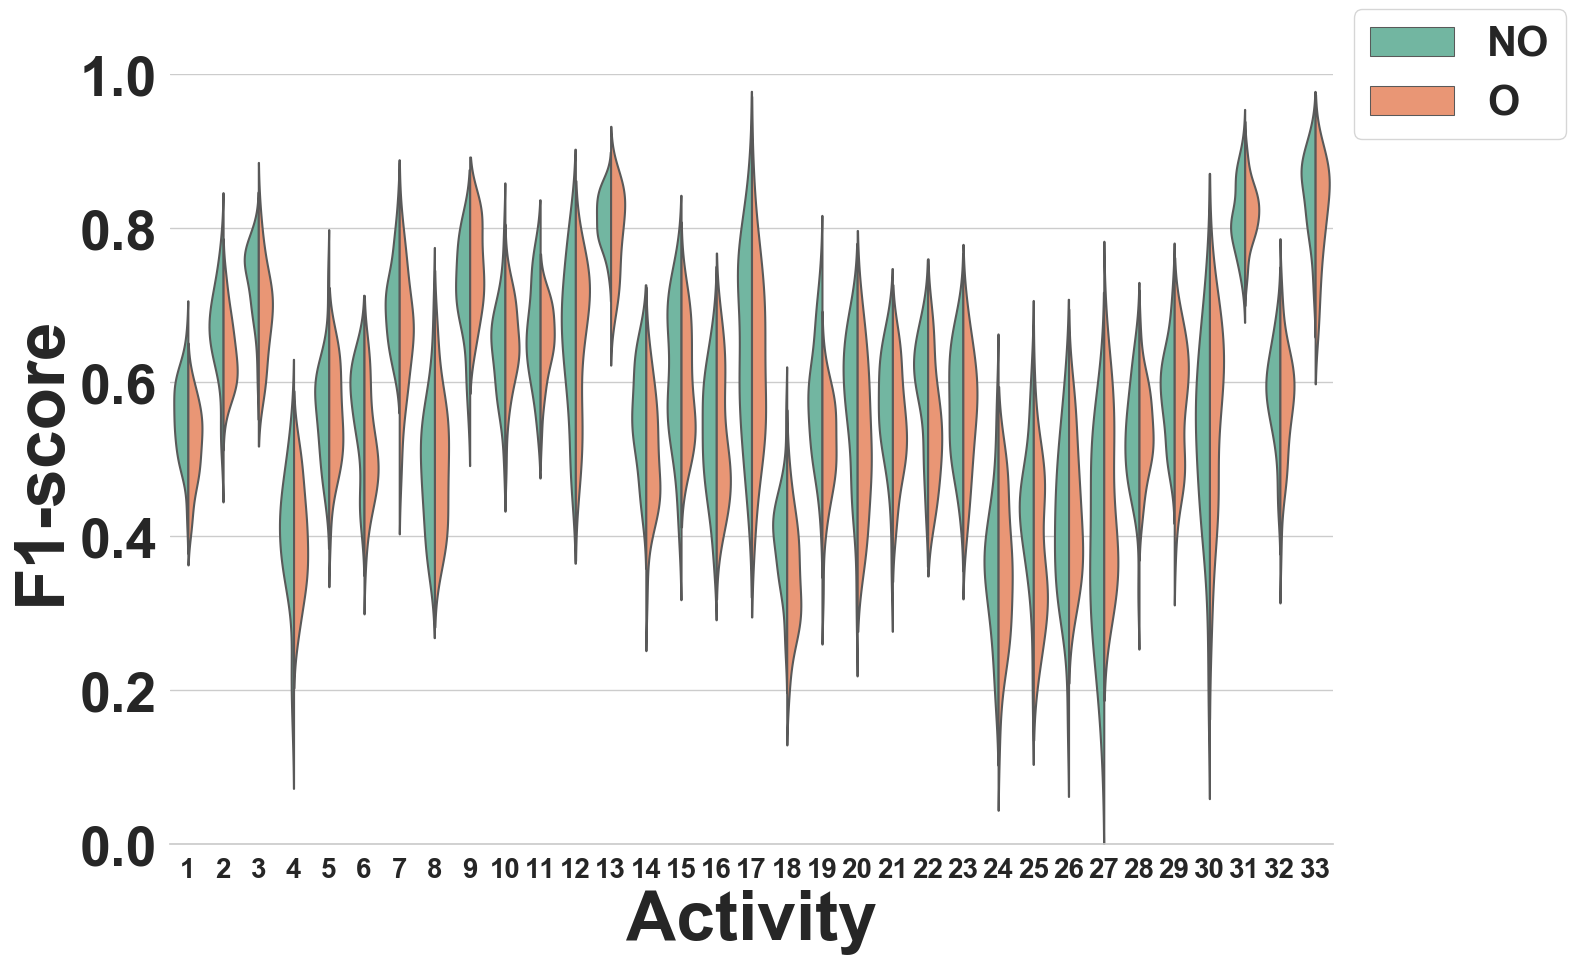
\includegraphics[scale=0.18]{Figures/per_activity_Dataset1_DT_sbj_FS3.png}}\quad
  \subfigure[KNN]{\label{fig:KNN_ds1-activity-exp5}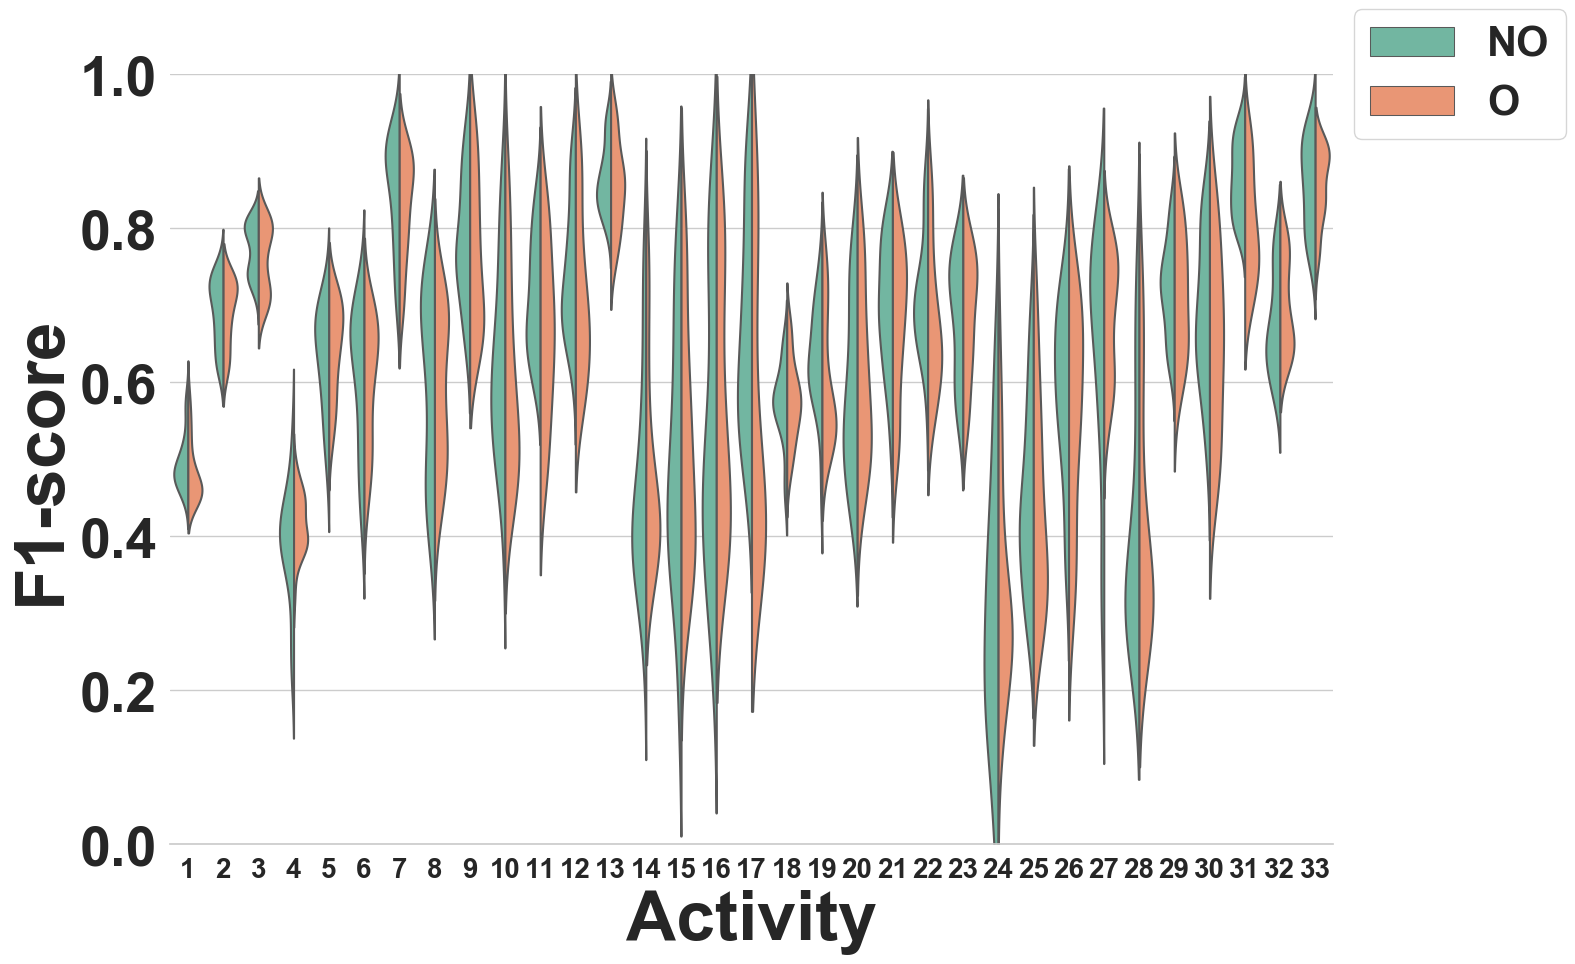
\includegraphics[scale=0.18]{Figures/per_activity_Dataset1_KNN_sbj_FS3.png}}
  \subfigure[NB]{\label{fig:NB_ds1-activity-exp5}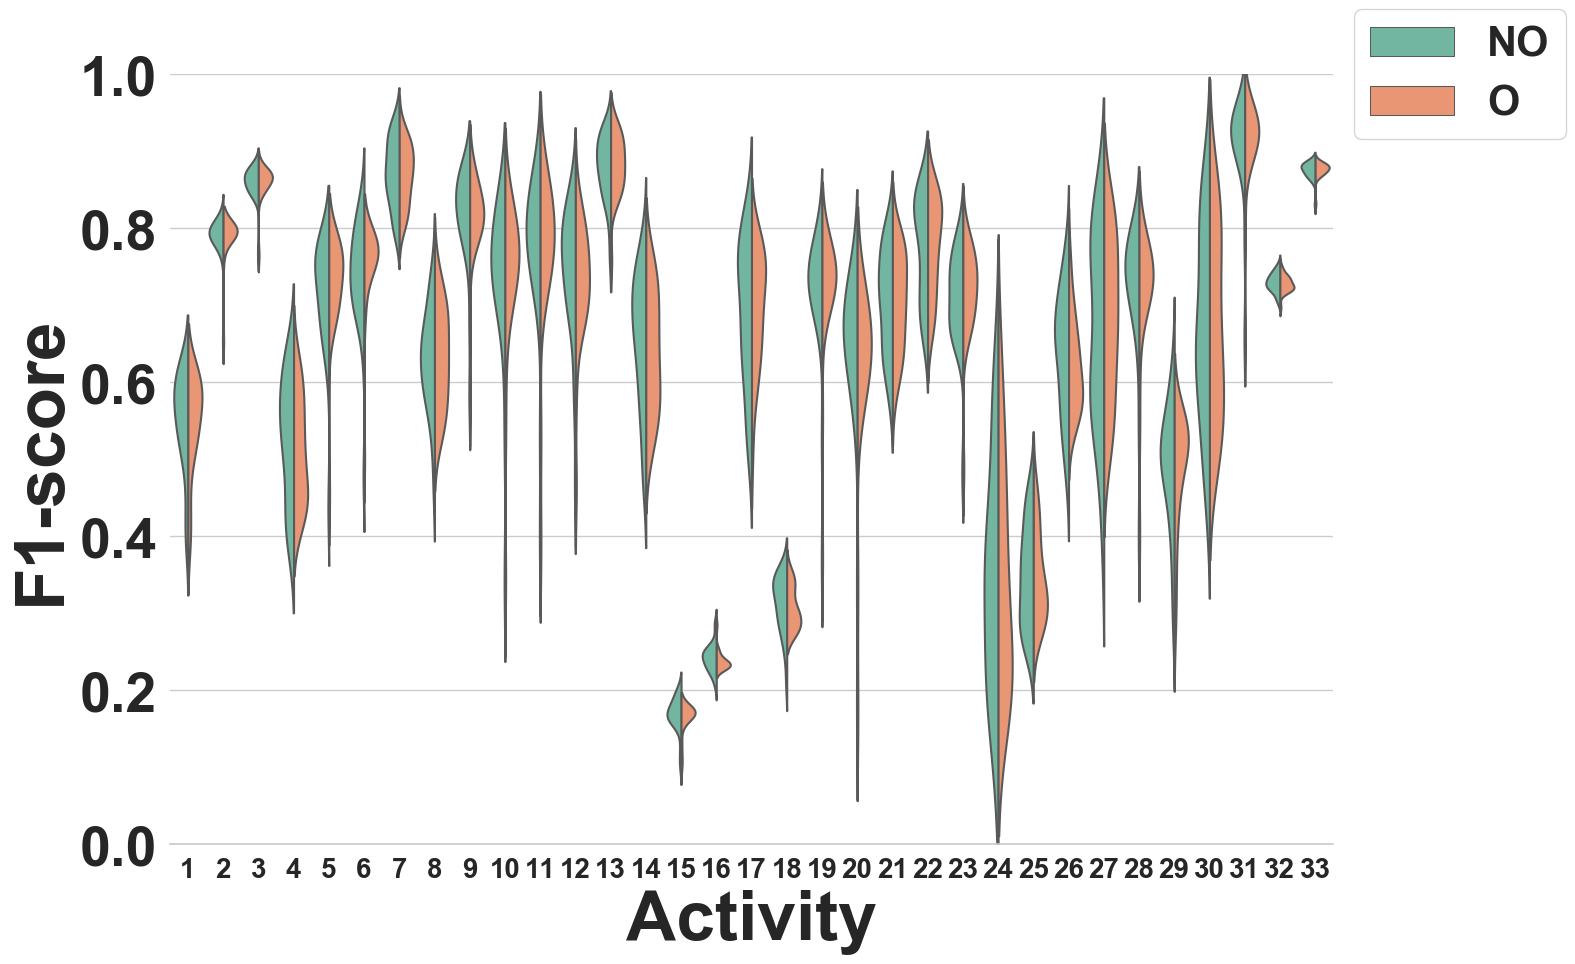
\includegraphics[scale=0.18]{Figures/per_activity_Dataset1_NB_sbj_FS3.png}}
    \subfigure[NCC]{\label{fig:NCC_ds1-activity-exp5}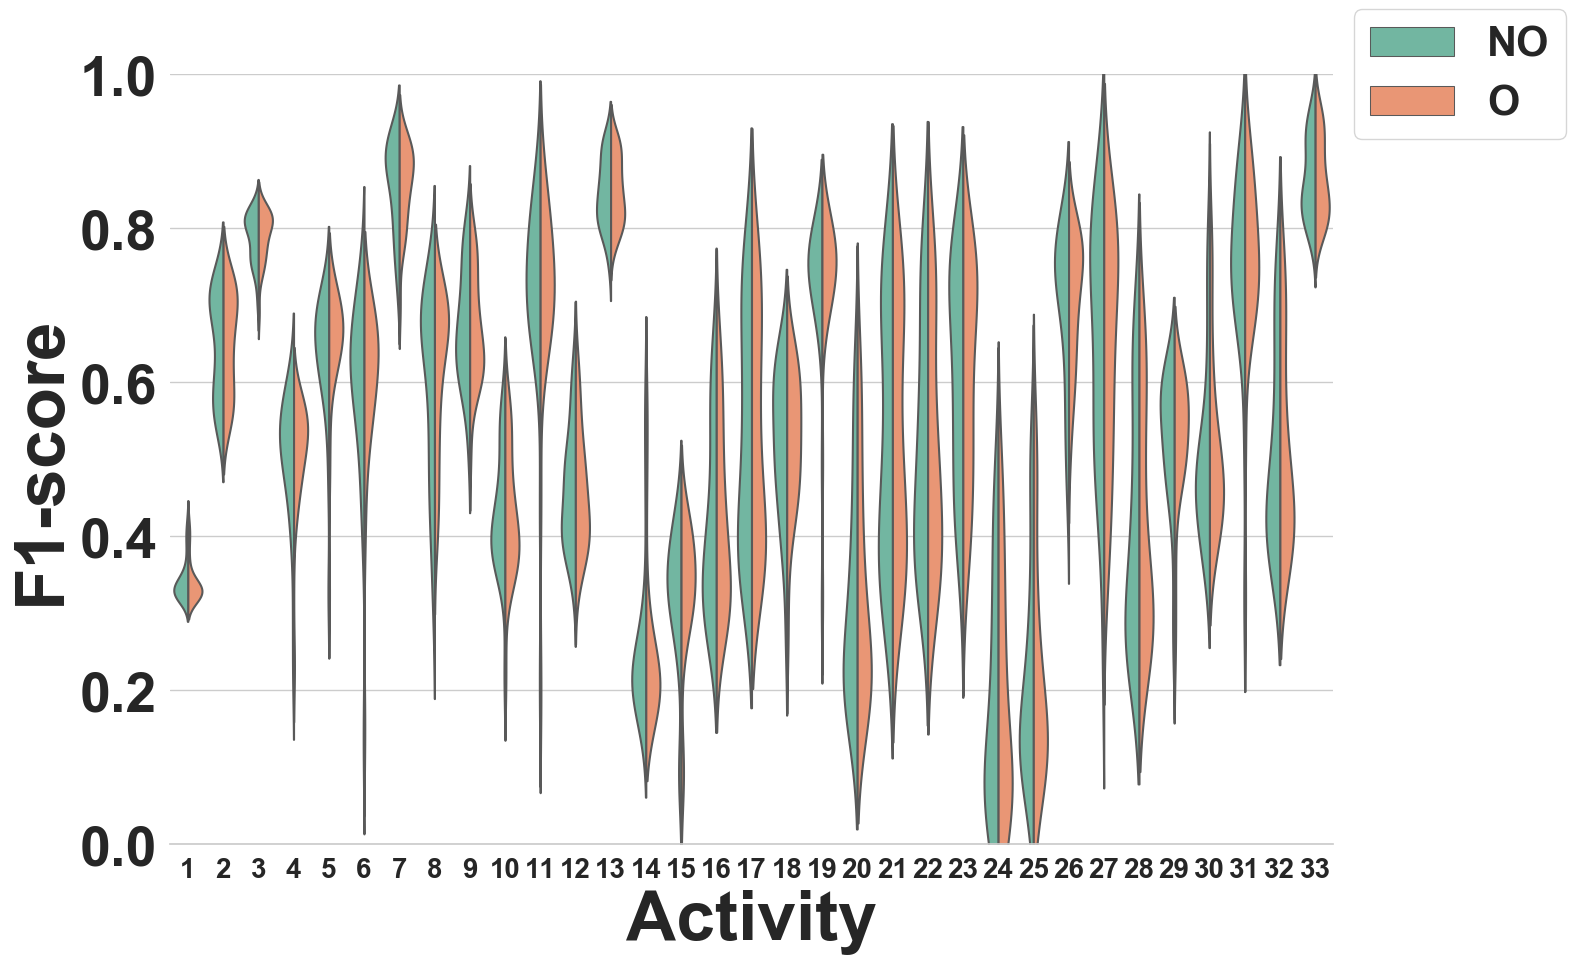
\includegraphics[scale=0.18]{Figures/per_activity_Dataset1_NCC_sbj_FS3.png}}
   
   \caption{Experiment 4 -- Subject-independent CV -- Dataset 1.}
    \label{fig:exp5_ds1}
    
\end{figure}

\begin{figure}[htp]
  \centering
  \subfigure[DT]{\label{fig:DT_ds2-activity-exp5}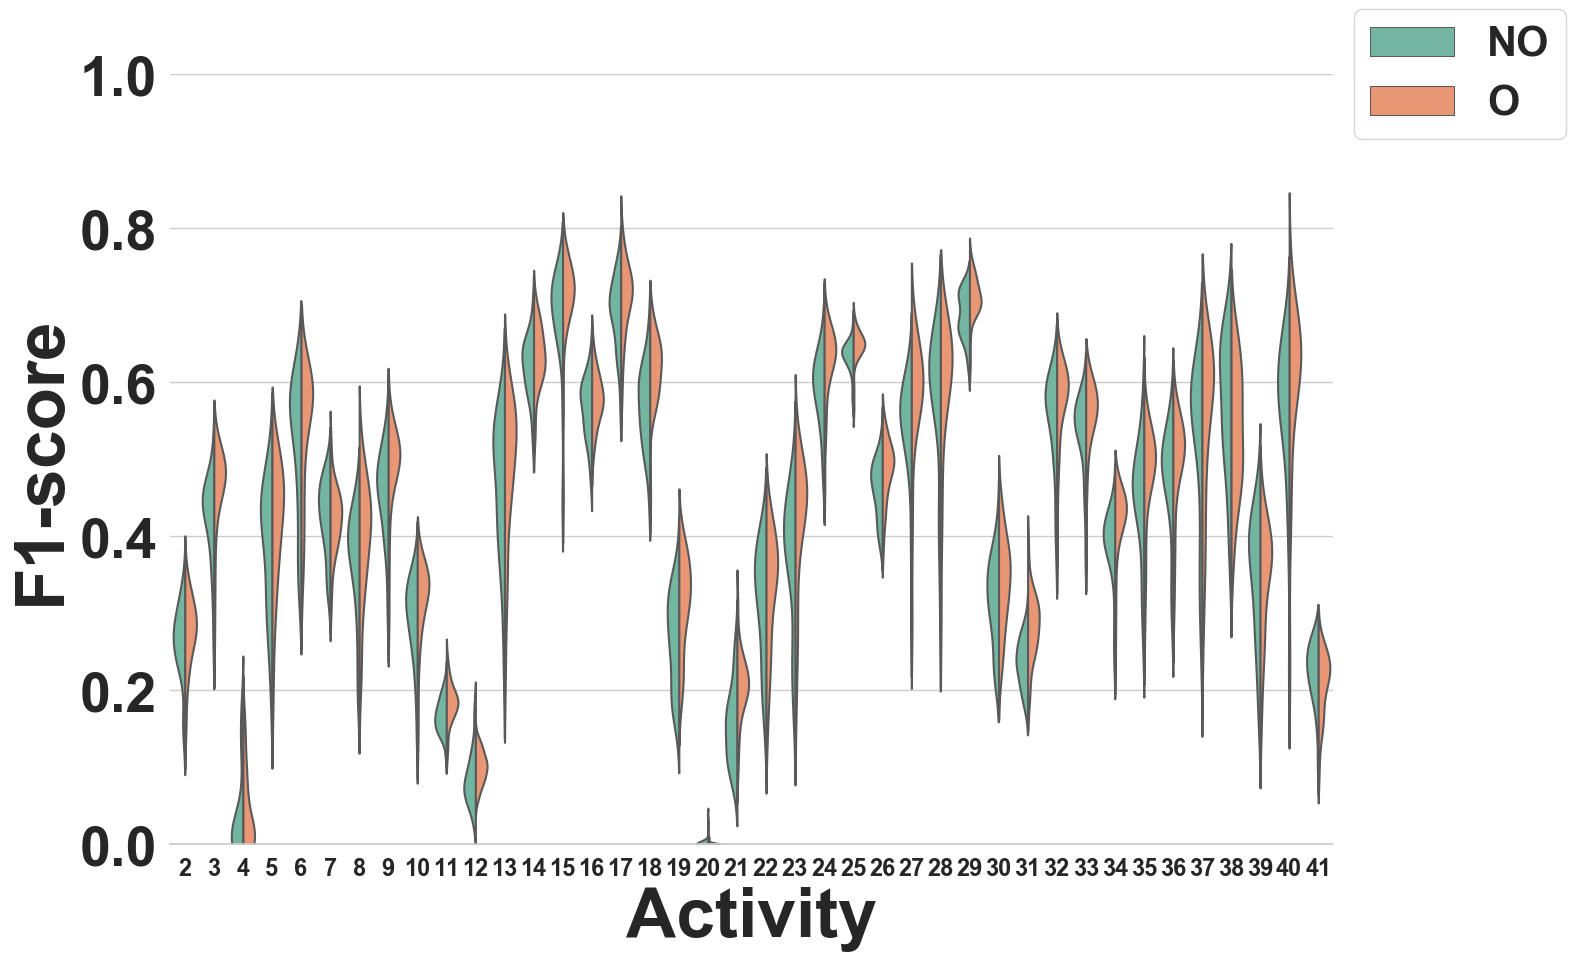
\includegraphics[scale=0.18]{Figures/per_activity_Dataset2_DT_sbj_FS3.png}}\quad
  \subfigure[KNN]{\label{fig:KNN_ds2-activity-exp5}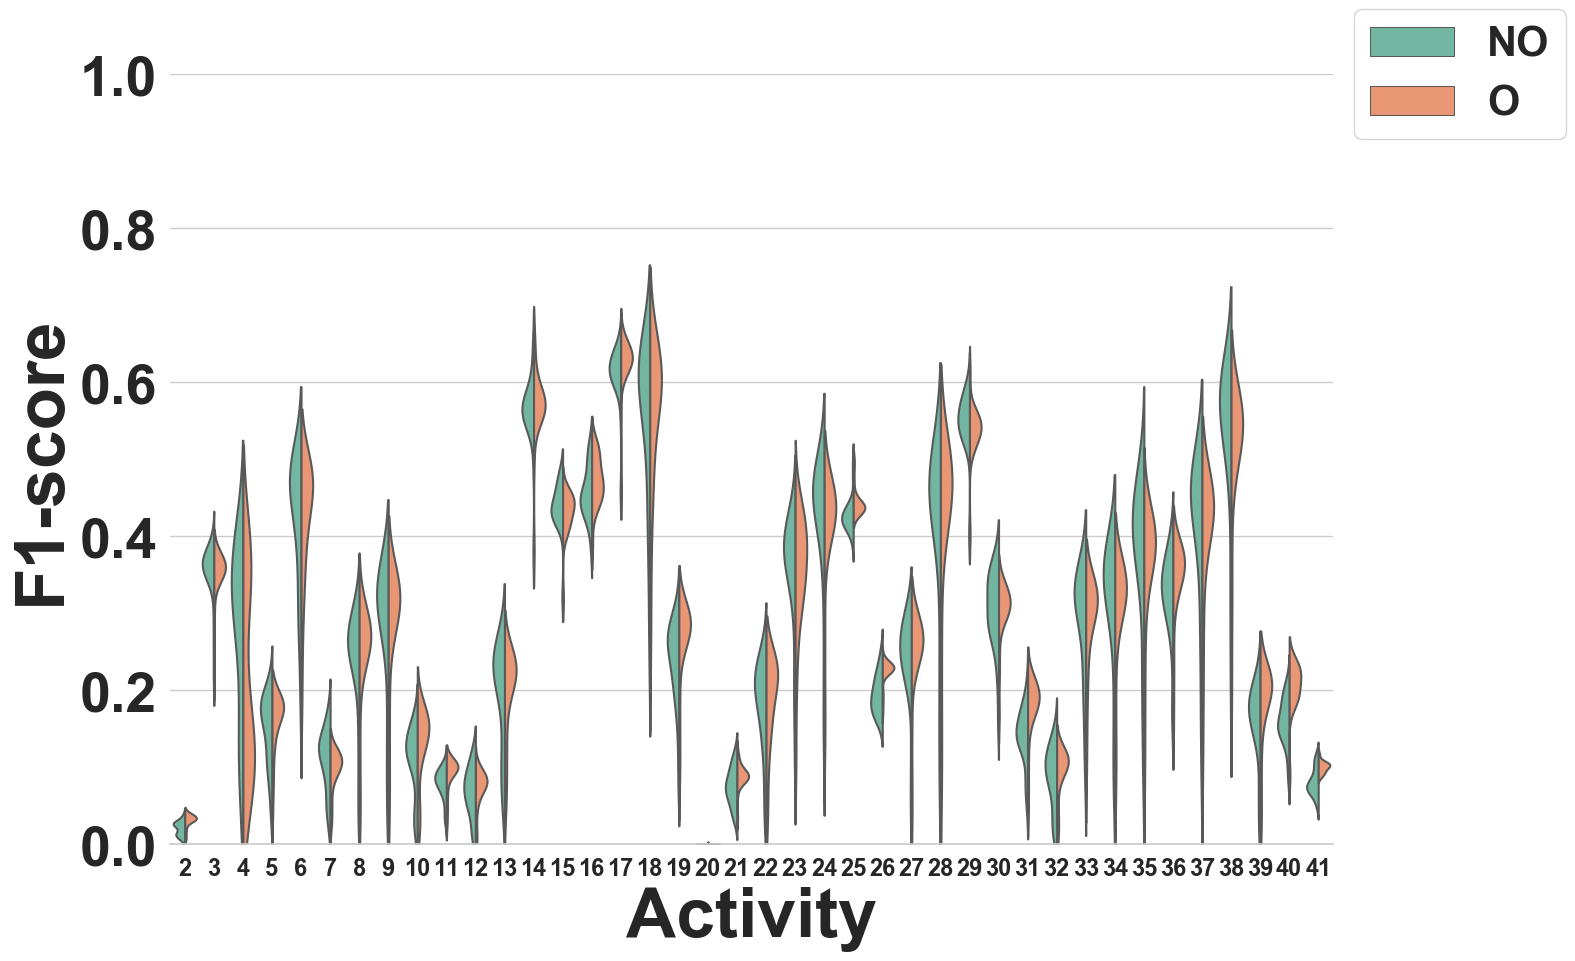
\includegraphics[scale=0.18]{Figures/per_activity_Dataset2_KNN_sbj_FS3.png}}
  \subfigure[NB]{\label{fig:NB_ds2-activity-exp3}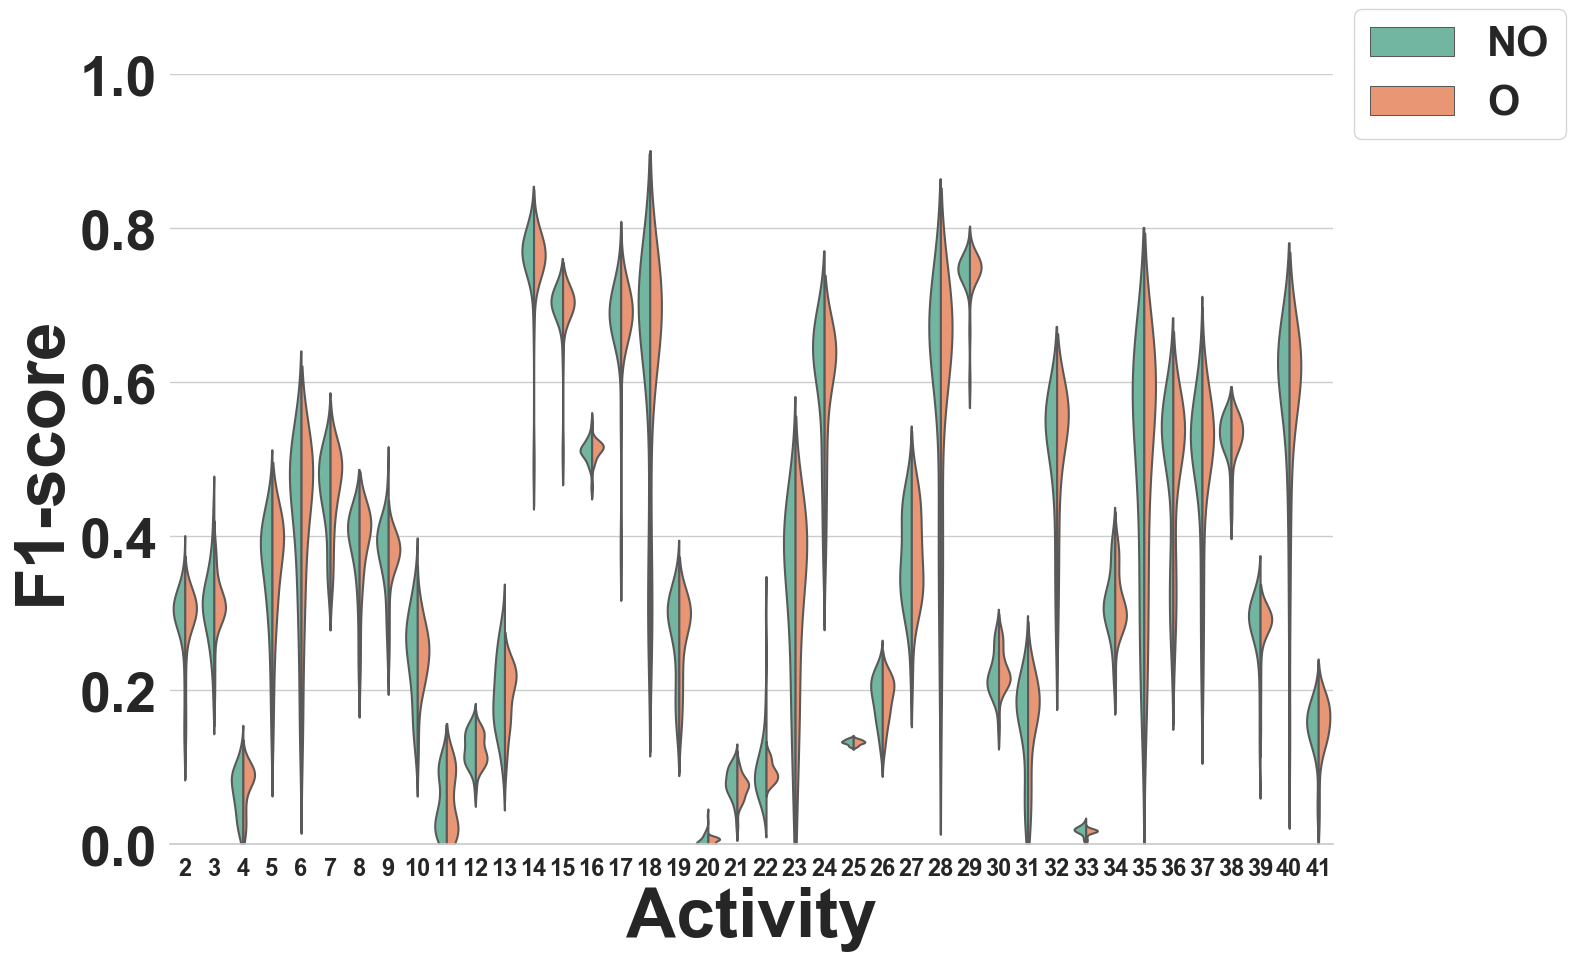
\includegraphics[scale=0.18]{Figures/per_activity_Dataset2_NB_sbj_FS3}}
    \subfigure[NCC]{\label{fig:NCC_ds2-activity-exp5}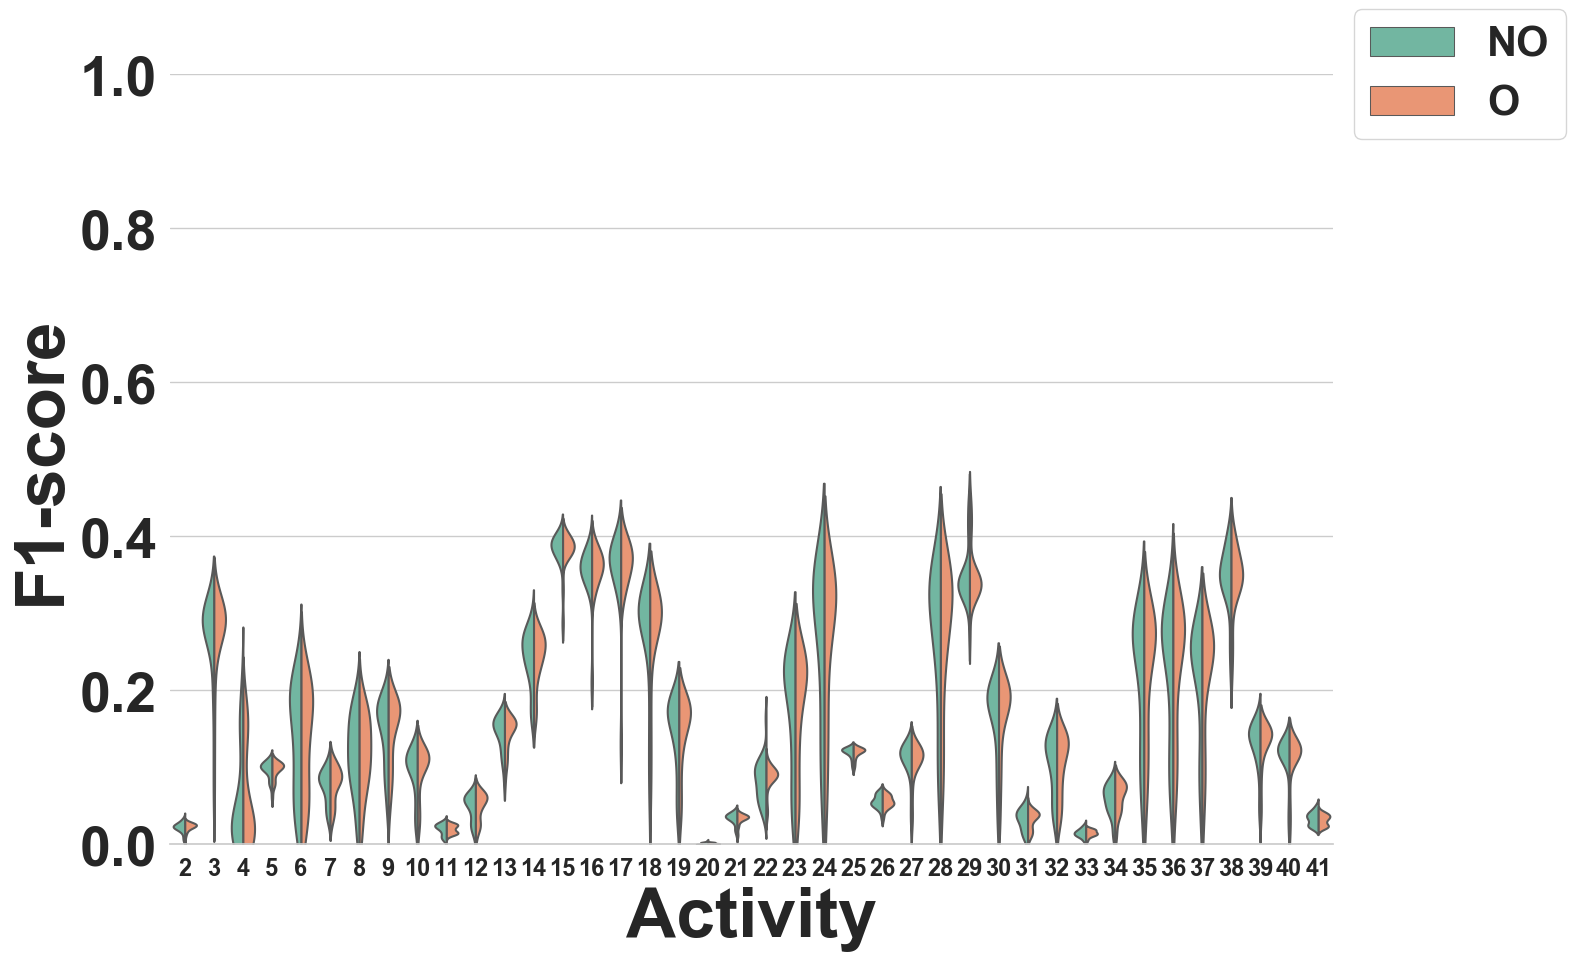
\includegraphics[scale=0.18]{Figures/per_activity_Dataset2_NCC_sbj_FS3.png}}
   
   \caption{Experiment 4 -- Subject-independent CV -- Dataset 2.}
    \label{fig:exp5_ds2}
    
\end{figure}
